\documentclass[11pt,a4paper]{article}
% >>> PERSONALIZZA <<<
\newcommand{\titolobreve}{Random Forest \,·\, Manuale teorico e pratico}  % testo dell'intestazione
\newcommand{\etichettasezione}{Capitolo}                  % oppure: Sezione

% ---------------- Matematica (Palatino, stile manuale scientifico) ----------------
\usepackage{amsmath,amssymb,mathtools}
\usepackage[sc]{mathpazo}
\usepackage{bm}
\linespread{1.06}

% ---------------- Font del testo ----------------
\usepackage[no-math]{fontspec}
\setmainfont{TeX Gyre Pagella}
\setsansfont{Fira Sans}[BoldFont={Fira Sans SemiBold},ItalicFont={Fira Sans Italic},BoldItalicFont={Fira Sans SemiBold Italic}]
\newfontfamily\headfont{Fira Sans}[BoldFont={Fira Sans SemiBold},ItalicFont={Fira Sans Italic}]
\newfontfamily\headlight{Fira Sans Light}
\newfontfamily\headblack{Fira Sans ExtraBold}

\usepackage{babel}
\babelprovide[import,main]{italian}

% ---------------- Pagina ----------------
\usepackage[a4paper,top=2.5cm,bottom=2.4cm,left=2.3cm,right=2.3cm,headheight=15pt,headsep=0.9cm]{geometry}
\usepackage[table]{xcolor}
\usepackage{graphicx,tikz,booktabs,array,tabularx,enumitem,ragged2e,pifont,microtype}
\usetikzlibrary{calc,positioning,shapes.geometric,arrows.meta,shadows}
\usepackage[most]{tcolorbox}
\usepackage{titlesec,fancyhdr,tocloft}
\usepackage[hidelinks]{hyperref}

\setlength{\parindent}{0pt}
\setlength{\parskip}{5pt plus 1pt}
\raggedright
\setlength{\RaggedRightParindent}{0pt}
\emergencystretch=2em

% ---------------- Palette ----------------
\definecolor{navy}{HTML}{1F3A5F}
\definecolor{teal}{HTML}{1B8A8A}
\definecolor{blu}{HTML}{2A6FDB}
\definecolor{rosso}{HTML}{E0533D}
\definecolor{ambra}{HTML}{D9940F}
\definecolor{viola}{HTML}{6B4FBB}
\definecolor{verde}{HTML}{2E9E5B}
\definecolor{grigio}{HTML}{5A6170}
\definecolor{chiaro}{HTML}{EEF2F7}
\definecolor{testo}{HTML}{22262D}
\color{testo}

% vettori in grassetto
\newcommand{\x}{\mathbf{x}}
\newcommand{\vv}{\mathbf{v}}
\newcommand{\mmu}{\bm{\mu}}
\newcommand{\SSigma}{\bm{\Sigma}}
\newcommand{\argmax}{\operatorname*{arg\,max}}
\newcommand{\T}{^{\mathsf{t}}}
\newcommand{\hl}[1]{{\color{navy}\bfseries #1}}
\newcommand{\key}[1]{\textcolor{teal}{\textbf{#1}}}
\newcommand{\slide}[1]{{\headfont\footnotesize\color{grigio}\,[slide #1]}}

% ---------------- Liste ----------------
\setlist{itemsep=2pt,topsep=3pt,parsep=0pt}
\setlist[itemize,1]{label={\color{teal}\small$\blacktriangleright$},leftmargin=1.3em}
\setlist[itemize,2]{label={\color{ambra}\footnotesize$\bullet$},leftmargin=1.2em}
\setlist[enumerate,1]{label={\headfont\bfseries\color{navy}\arabic*.},leftmargin=1.6em}

% ---------------- Icone (tikz) ----------------
\newcommand{\iconbulb}{\tikz[baseline=-0.6ex,scale=.85]{\fill[white](0,.06)circle(.13);\fill[white](-.07,-.15)rectangle(.07,-.06);\draw[white,line width=.4pt](-.06,-.19)--(.06,-.19);}}
\newcommand{\iconwarn}{\tikz[baseline=-0.6ex]{\node[regular polygon,regular polygon sides=3,fill=white,inner sep=1.1pt,minimum size=11pt]{}; \node[font=\headblack\tiny,text=rosso] at (0,-.02){!};}}
\newcommand{\iconml}{\tikz[baseline=-0.6ex,scale=.8]{\foreach \y in {-.16,.16}{\fill[white](-.2,\y)circle(.05);} \foreach \y in {-.2,0,.2}{\fill[white](.2,\y)circle(.05);\draw[white,line width=.35pt](-.2,.16)--(.2,\y);\draw[white,line width=.35pt](-.2,-.16)--(.2,\y);}}}

% ---------------- Box ----------------
\tcbset{every box/.style={halign=flush left}}
\tcbset{
  base/.style={enhanced,breakable,arc=3pt,boxrule=0pt,left=11pt,right=11pt,top=9pt,bottom=8pt,
    before skip=12pt,after skip=12pt,fonttitle=\headfont\bfseries\small,
    attach boxed title to top left={xshift=10pt,yshift=-9pt},
    boxed title style={arc=2.5pt,boxrule=0pt,left=6pt,right=6pt,top=2pt,bottom=2pt},
    overlay unbroken and first={}},
}
\newtcolorbox{intuizione}[1][Intuizione]{base,colback=teal!6,colbacktitle=teal,coltitle=white,
  borderline west={3pt}{0pt}{teal},title={\iconbulb\ \ #1},top=13pt}
\newtcolorbox{tecnica}[1][In termini tecnici]{base,colback=navy!5,colbacktitle=navy,coltitle=white,
  borderline west={3pt}{0pt}{navy},title={$\Sigma$\ \ #1},top=13pt}
\newtcolorbox{esempio}[1][Esempio]{base,colback=ambra!7,colbacktitle=ambra,coltitle=white,
  borderline west={3pt}{0pt}{ambra},title={\ding{46}\ \ #1},top=13pt}
\newtcolorbox{attenzione}[1][Attenzione]{base,colback=rosso!6,colbacktitle=rosso,coltitle=white,
  borderline west={3pt}{0pt}{rosso},title={\iconwarn\ \ #1},top=13pt}
\newtcolorbox{mlbox}[1][Approfondimento]{base,colback=viola!6,colbacktitle=viola,coltitle=white,
  borderline west={3pt}{0pt}{viola},title={\iconml\ \ #1},top=13pt}
\newtcolorbox{formula}[1][]{enhanced,arc=5pt,boxrule=0.9pt,colframe=navy!55,colback=white,
  left=8pt,right=8pt,top=6pt,bottom=6pt,before skip=10pt,after skip=10pt,halign=flush center,
  #1}
\newtcolorbox{formulat}[1]{enhanced,arc=5pt,boxrule=0.9pt,colframe=navy!55,colback=white,
  left=8pt,right=8pt,top=10pt,bottom=6pt,before skip=14pt,after skip=10pt,halign=flush center,
  attach boxed title to top center={yshift=-8pt},boxed title style={colback=navy!55,arc=2pt,boxrule=0pt,top=1pt,bottom=1pt},
  fonttitle=\headfont\bfseries\footnotesize,coltitle=white,title={#1}}
\newtcolorbox{appunti}[1]{enhanced,breakable,arc=4pt,boxrule=.8pt,colframe=grigio!60,colback=chiaro,
  left=12pt,right=12pt,top=12pt,bottom=10pt,before skip=16pt,after skip=8pt,
  fonttitle=\headfont\bfseries\small,coltitle=white,colbacktitle=grigio,
  attach boxed title to top left={xshift=10pt,yshift=-9pt},boxed title style={arc=2.5pt,boxrule=0pt,left=6pt,right=6pt},
  title={\ding{43}\ \ #1},fontupper=\small}
\newcommand{\pag}[1]{\par\vspace{4pt}{\headfont\bfseries\scriptsize\setlength{\fboxsep}{1.5pt}\colorbox{teal}{\color{white}\,p.\,#1\,}}\enspace}

% ---------------- Titoli ----------------
\newcounter{sez}
\newcommand{\sezione}[3]{% num titolo slide
  \clearpage
  \refstepcounter{section}
  \addcontentsline{toc}{section}{\protect\numberline{\thesection}#2}
  \markboth{#2}{#2}
  \begin{tikzpicture}
    \fill[navy,rounded corners=8pt] (0,0) rectangle (\textwidth,2.6cm);
    \fill[teal,rounded corners=8pt] (0,0) rectangle (2.6cm,2.6cm);
    \fill[teal] (1.6cm,0) rectangle (2.6cm,2.6cm);
    \node[font=\headblack\fontsize{40}{40}\selectfont,text=white] at (1.3cm,1.3cm) {\thesection};
    \node[anchor=south west,font=\headfont\bfseries\fontsize{19}{22}\selectfont,text=white,text width=\textwidth-3.6cm,align=left] at (3.0cm,.85cm) {#2};
    \node[anchor=west,font=\headlight\small,text=white!80!teal] at (3.1cm,.48cm) {\etichettasezione\ #1 \quad·\quad #3};
  \end{tikzpicture}
  \par\vspace{6pt}
}
\titleformat{\subsection}{\headfont\bfseries\large\color{navy}}{\colorbox{teal!15}{\color{teal}\thesubsection}}{0.6em}{}
\titlespacing*{\subsection}{0pt}{16pt}{6pt}
\titleformat{\subsubsection}{\headfont\bfseries\normalsize\color{teal}}{}{0em}{}
\titlespacing*{\subsubsection}{0pt}{10pt}{3pt}

% ---------------- Header / footer ----------------
\pagestyle{fancy}
\fancyhf{}
\renewcommand{\headrulewidth}{0pt}
\fancyhead[L]{\headfont\footnotesize\color{grigio}\titolobreve}
\fancyhead[R]{\headfont\footnotesize\color{teal}\leftmark}
\fancyfoot[C]{\tikz{\node[circle,fill=navy,text=white,font=\headfont\bfseries\footnotesize,minimum size=17pt,inner sep=0pt]{\thepage};}}
\fancypagestyle{plain}{\fancyhf{}\fancyfoot[C]{\tikz{\node[circle,fill=navy,text=white,font=\headfont\bfseries\footnotesize,minimum size=17pt,inner sep=0pt]{\thepage};}}}

% ---------------- Indice ----------------
\renewcommand{\cfttoctitlefont}{\headfont\bfseries\Huge\color{navy}}
\renewcommand{\cftsecfont}{\headfont\bfseries\color{navy}}
\renewcommand{\cftsecpagefont}{\headfont\bfseries\color{teal}}
\renewcommand{\cftsecleader}{\color{grigio!50}\cftdotfill{\cftdotsep}}
\renewcommand{\cftsubsecfont}{\headfont\small\color{grigio}}
\renewcommand{\cftsubsecpagefont}{\headfont\small\color{grigio}}
\setlength{\cftbeforesecskip}{7pt}
\setcounter{tocdepth}{1}

% tabelle
\newcommand{\thd}[1]{{\headfont\bfseries\small\color{white}#1}}
\renewcommand{\arraystretch}{1.25}
\renewcommand{\tabularxcolumn}[1]{m{#1}}
\newcolumntype{Y}{>{\raggedright\arraybackslash}X}
\newcommand{\fig}[2][\linewidth]{\begin{center}\includegraphics[width=#1]{figs/#2}\end{center}}
\newcommand{\didascalia}[1]{\vspace{-8pt}\begin{center}\begin{minipage}{.9\linewidth}\centering\headfont\footnotesize\color{grigio}#1\end{minipage}\end{center}\vspace{-2pt}}


% ---------------- Codice e terminali ----------------
\setmonofont{DejaVu Sans Mono}[Scale=0.84]
\usepackage{listings}
\definecolor{termbg}{HTML}{14202E}
\definecolor{termfg}{HTML}{E4E9F0}
\definecolor{termprompt}{HTML}{5FD3B4}
\definecolor{termhl}{HTML}{F5C04A}
\definecolor{termdim}{HTML}{8A97A8}
\lstdefinestyle{term}{basicstyle=\ttfamily\small\color{termfg},columns=fullflexible,keepspaces=true,
  breaklines=true,breakatwhitespace=false,postbreak=\mbox{\textcolor{termdim}{$\hookrightarrow$}\space},
  showstringspaces=false,upquote=true,
  moredelim=[is][\color{termprompt}\bfseries]{§}{§},
  moredelim=[is][\color{termhl}\bfseries]{¤}{¤},
  moredelim=[is][\color{termdim}\itshape]{°}{°},
  literate={à}{{\`a}}1 {è}{{\`e}}1 {é}{{\'e}}1 {ì}{{\`i}}1 {ò}{{\`o}}1 {ù}{{\`u}}1}
\lstdefinestyle{file}{basicstyle=\ttfamily\small\color{testo},columns=fullflexible,keepspaces=true,breaklines=true,
  upquote=true,showstringspaces=false,
  moredelim=[is][\color{teal}\bfseries]{§}{§},
  moredelim=[is][\color{rosso}\bfseries]{¤}{¤},
  moredelim=[is][\color{grigio}\itshape]{°}{°},
  literate={à}{{\`a}}1 {è}{{\`e}}1 {é}{{\'e}}1 {ì}{{\`i}}1 {ò}{{\`o}}1 {ù}{{\`u}}1}
\tcbuselibrary{listings}
% terminale: argomento = titolo della finestra
\newtcblisting{terminale}[1]{enhanced,listing only,breakable,colback=termbg,colframe=termbg,arc=5pt,boxrule=0pt,
  left=9pt,right=9pt,top=4pt,bottom=4pt,before skip=9pt,after skip=9pt,
  listing options={style=term},
  title={\tikz[baseline=-.6ex]{\foreach \c [count=\i] in {rosso,ambra,verde}{\fill[\c](\i*.32,0)circle(.09);}}\hfill{\ttfamily\footnotesize\color{termdim}\detokenize{#1}}\hfill\phantom{\tikz{\fill(0,0)circle(.09);\fill(.64,0)circle(.09);}}},
  colbacktitle=termbg!80!white,coltitle=white,toptitle=3pt,bottomtitle=3pt,titlerule=0pt}
% file di configurazione: argomento = nome del file
\newtcblisting{filecfg}[1]{enhanced,listing only,breakable,colback=white,colframe=navy!40,arc=4pt,boxrule=.7pt,
  left=9pt,right=9pt,top=4pt,bottom=4pt,before skip=9pt,after skip=9pt,listing options={style=file},
  attach boxed title to top left={xshift=8pt,yshift=-8pt},boxed title style={colback=navy!70,arc=2pt,boxrule=0pt},
  fonttitle=\ttfamily\footnotesize\bfseries,coltitle=white,title={#1},top=10pt}
\newcommand{\cmd}[1]{\texttt{\color{navy}#1}}
\newcommand{\inl}[1]{{\setlength{\fboxsep}{1.2pt}\colorbox{chiaro}{\ttfamily\small\color{navy}#1}}}
% scheda comando
\newtcolorbox{scheda}[2][]{enhanced,breakable,arc=4pt,boxrule=0pt,colback=white,
  borderline={.8pt}{0pt}{teal!60},left=11pt,right=11pt,top=10pt,bottom=8pt,before skip=14pt,after skip=12pt,
  title={\ttfamily\bfseries\normalsize #2},fonttitle=\color{white},colbacktitle=teal,
  toptitle=4pt,bottomtitle=4pt,#1}
\newcommand{\campo}[1]{\par\vspace{3pt}{\headfont\bfseries\footnotesize\color{teal}\MakeUppercase{#1}}\par\vspace{1pt}}
\tikzset{
  dev/.style={draw=navy,fill=white,line width=1pt,rounded corners=3pt,minimum width=1.25cm,minimum height=.75cm,font=\headfont\bfseries\small,text=navy},
  host/.style={dev,fill=blu!8,draw=blu},
  rtr/.style={circle,draw=teal,fill=teal!10,line width=1.1pt,minimum size=1.05cm,font=\headfont\bfseries\small,text=teal!70!black},
  cd/.style={draw=ambra,fill=ambra!15,line width=1pt,rounded corners=7pt,minimum width=1.0cm,minimum height=.62cm,font=\headfont\bfseries,text=ambra!60!black},
  lnk/.style={line width=1.2pt,color=grigio!80},
  lab/.style={font=\ttfamily\scriptsize,text=testo,fill=white,inner sep=1.2pt,rounded corners=1pt},
  ipl/.style={font=\ttfamily\scriptsize\bfseries,text=rosso!85!black,fill=white,inner sep=1.2pt},
  macl/.style={font=\ttfamily\scriptsize,text=viola,fill=viola!8,inner sep=1.5pt,rounded corners=1pt},
  netl/.style={font=\ttfamily\scriptsize\bfseries,text=verde!70!black,fill=verde!8,draw=verde!50,rounded corners=2pt,inner sep=2pt},
}
\newcommand{\wsrow}[7]{\rowcolor{#7}#1 & #2 & #3 & #4 & #5 & #6\\}

\newcommand{\sint}[1]{{\ttfamily\small\color{navy}\raggedright #1\par}}


% ---------------- Codice Python (aggiunta per questo manuale) ----------------
\definecolor{pykw}{HTML}{1F3A5F}
\definecolor{pystr}{HTML}{2E7D4F}
\definecolor{pycom}{HTML}{7A8290}
\definecolor{pybg}{HTML}{F7F9FC}
\lstdefinestyle{py}{language=Python,basicstyle=\ttfamily\small\color{testo},columns=fullflexible,keepspaces=true,
  breaklines=true,upquote=true,showstringspaces=false,
  keywordstyle=\color{pykw}\bfseries,stringstyle=\color{pystr},commentstyle=\color{pycom}\itshape,
  morekeywords={as,with,None,True,False,self},
  emph={RandomForestClassifier,RandomForestRegressor,Pipeline,GridSearchCV,train_test_split,cross_val_score,
        StratifiedKFold,SimpleImputer,permutation_importance,DecisionTreeRegressor,LinearRegression,RepeatedKFold,
        ColumnTransformer,OneHotEncoder,RandomizedSearchCV},emphstyle=\color{teal}\bfseries,
  numbers=left,numberstyle=\tiny\color{grigio!70},numbersep=7pt,xleftmargin=12pt,
  literate={à}{{\`a}}1 {è}{{\`e}}1 {é}{{\'e}}1 {ì}{{\`i}}1 {ò}{{\`o}}1 {ù}{{\`u}}1}
% codice: argomento = nome del file
\newtcblisting{codice}[1]{enhanced,listing only,breakable,colback=pybg,colframe=teal!55,arc=4pt,boxrule=.7pt,
  left=4pt,right=8pt,top=10pt,bottom=4pt,before skip=12pt,after skip=10pt,listing options={style=py},
  attach boxed title to top left={xshift=8pt,yshift=-8pt},boxed title style={colback=teal,arc=2pt,boxrule=0pt},
  fonttitle=\ttfamily\footnotesize\bfseries,coltitle=white,title={\ding{230}\ \detokenize{#1}}}
% riga di codice richiamata nel testo
\newcommand{\riga}[1]{{\headfont\bfseries\scriptsize\setlength{\fboxsep}{1.4pt}\colorbox{teal!15}{\color{teal!70!black}r.\,#1}}}
\newcommand{\E}{\mathbb{E}}
\newcommand{\Var}{\operatorname{Var}}
\newcommand{\Corr}{\operatorname{Corr}}
\newcommand{\argmin}{\operatorname*{arg\,min}}

% ---------------- Elementi per manuali senza formule/codice ----------------
\newtcolorbox{consiglio}[1][Consiglio]{base,colback=verde!6,colbacktitle=verde,coltitle=white,
  borderline west={3pt}{0pt}{verde},title={\ding{51}\ \ #1},top=13pt}
% passi numerati con cerchi (procedure, istruzioni d'uso)
\newlist{passi}{enumerate}{1}
\setlist[passi]{label={\protect\tikz[baseline=(n.base)]\protect\node[circle,fill=teal,text=white,font=\headfont\bfseries\footnotesize,inner sep=0pt,minimum size=1.35em](n){\arabic*};},leftmargin=2.1em,itemsep=6pt,topsep=6pt}
% box «In breve» per riassunti di poche righe in apertura di capitolo
\newtcolorbox{inbreve}{enhanced,arc=4pt,boxrule=0pt,colback=chiaro,left=12pt,right=12pt,top=8pt,bottom=8pt,
  borderline north={2pt}{0pt}{teal},fontupper=\small,before skip=6pt,after skip=10pt}
\tcbset{codicestyle/.style={enhanced,listing only,breakable,colback=pybg,colframe=teal!55,arc=4pt,boxrule=.7pt,
  left=4pt,right=8pt,top=10pt,bottom=4pt,before skip=12pt,after skip=10pt,listing options={style=py},
  attach boxed title to top left={xshift=8pt,yshift=-8pt},boxed title style={colback=teal,arc=2pt,boxrule=0pt},
  fonttitle=\ttfamily\footnotesize\bfseries,coltitle=white}}
% \codicefile{file}{prima riga}{ultima riga}
\newcommand{\codicefile}[3]{\tcbinputlisting{codicestyle,listing file=code/#1,
  listing options={style=py,firstline=#2,lastline=#3,firstnumber=#2},title={\ding{230}\ \detokenize{#1}\ \ (righe #2--#3)}}}

\begin{document}
% ================= COPERTINA =================
\thispagestyle{empty}
\begin{tikzpicture}[remember picture,overlay]
  \fill[navy] (current page.north west) rectangle ([yshift=-15.5cm]current page.north east);
  \fill[teal] ([yshift=-15.5cm]current page.north west) rectangle ([yshift=-16.1cm]current page.north east);
  \node[anchor=north west,font=\headfont\small\bfseries,text=ambra] at ([xshift=2.3cm,yshift=-2.2cm]current page.north west) {MACHINE LEARNING \,·\, METODI ENSEMBLE};
  \node[anchor=north west,font=\headblack\fontsize{48}{52}\selectfont,text=white,align=left] at ([xshift=2.2cm,yshift=-3.0cm]current page.north west) {Random\\[2pt]Forest};
  \node[anchor=north west,font=\headlight\Large,text=white!85!teal,align=left] at ([xshift=2.3cm,yshift=-7.1cm]current page.north west) {Dall'idea alla matematica, fino al codice\\in Python con scikit-learn};
  % motivo: una foresta di alberi stilizzati che "votano"
  \begin{scope}[shift={([xshift=2.6cm,yshift=-14.3cm]current page.north west)}]
    \foreach \x/\h/\o in {0/2.4/.16,1.55/3.3/.22,3.1/2.0/.14,4.65/3.8/.25,6.2/2.7/.18,7.75/3.5/.22,9.3/2.2/.15,10.85/3.1/.2,12.4/2.6/.17}{
      \fill[white,opacity=.25] (\x+.5,0) rectangle ++(.16,.55);
      \fill[white,opacity=\o] (\x,.5) -- (\x+.58,.5+\h) -- (\x+1.16,.5) -- cycle;
      \fill[white,opacity=\o] (\x+.1,.5+.45*\h) -- (\x+.58,.5+1.05*\h) -- (\x+1.06,.5+.45*\h) -- cycle;}
    \foreach \x/\c in {0/teal,1.55/rosso,3.1/teal,4.65/teal,6.2/rosso,7.75/teal,9.3/teal,10.85/rosso,12.4/teal}{
      \fill[\c!70!white] (\x+.58,-.45) circle (.13);}
    \draw[ambra,line width=1.2pt,-{Stealth[length=6pt]}] (0.58,-.8) -- (13.0,-.8);
    \node[font=\headfont\bfseries\footnotesize,text=ambra,anchor=west] at (13.1,-.8) {voto};
  \end{scope}
\end{tikzpicture}
\vspace*{15.2cm}
\begin{center}
\begin{tcolorbox}[enhanced,width=.8\linewidth,colback=white,colframe=navy!35,arc=6pt,boxrule=.8pt,halign=flush center,top=8pt,bottom=8pt]
\Large $\displaystyle \hat f_{\mathrm{rf}}(\x)=\frac{1}{B}\sum_{b=1}^{B} T_b\big(\x;\,\Theta_b\big)$\\[4pt]
{\headfont\small\color{grigio} molti alberi diversi, ognuno un po' sbagliato: la loro media sbaglia molto meno}
\end{tcolorbox}
\vspace{.8cm}
{\headfont\large\color{navy}\bfseries Manuale di studio teorico e pratico\par}
\vspace{2pt}
{\headfont\color{grigio}Codice verificato con Python 3 e scikit-learn 1.9 \,·\, A.A. 2026--2027\par}
\vspace{.9cm}
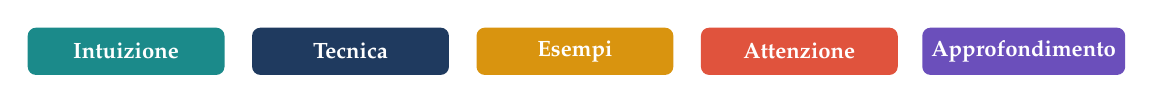
\begin{tikzpicture}
  \foreach \c/\t [count=\i] in {teal/Intuizione,navy/Tecnica,ambra/Esempi,rosso/Attenzione,viola/Approfondimento}{
    \node[fill=\c,text=white,font=\headfont\bfseries\footnotesize,rounded corners=3pt,minimum width=2.5cm,minimum height=.6cm] at (\i*2.85,0) {\t};}
\end{tikzpicture}
\end{center}
% ================= COME USARE =================
\clearpage\thispagestyle{plain}
{\headfont\bfseries\Huge\color{navy}Come usare questo manuale\par}
\vspace{4pt}{\color{teal}\rule{3cm}{2.5pt}}\vspace{8pt}

Il manuale è diviso in tre parti. La \hl{Parte I} (capitoli 1--6) costruisce il Random Forest un mattone alla volta: l'idea, gli alberi di decisione, il bootstrap, la casualità sulle feature, gli iperparametri e l'importanza delle variabili. La \hl{Parte II} (capitolo 7) spiega \hl{quali librerie usare e come organizzare il codice}. La \hl{Parte III} (capitoli 8--11) contiene quattro esempi completi, commentati riga per riga, e il capitolo 12 dice quando usare (e quando no) il Random Forest. In fondo trovi il \hl{formulario} e le \hl{fonti}.

Ogni argomento è spiegato due volte: prima l'\key{idea}, poi la \key{versione precisa}. I riquadri hanno sempre lo stesso significato:
\begin{intuizione}L'idea di fondo, con analogie e senza formule.\end{intuizione}
\begin{tecnica}Definizioni, formule e passaggi matematici.\end{tecnica}
\begin{esempio}Esempi svolti: tutti i numeri sono stati ricalcolati in Python.\end{esempio}
\begin{attenzione}Errori tipici, trappole e punti in cui le fonti non coincidono.\end{attenzione}
\begin{consiglio}Buone abitudini pratiche quando scrivi codice.\end{consiglio}
\begin{mlbox}Collegamenti, curiosità e uso nel mondo reale.\end{mlbox}
\begin{codice}{nome_file.py}
# Codice Python: i numeri a sinistra sono le righe,
# richiamate nel testo con le etichette  r. 12
\end{codice}
\begin{terminale}{output}
L'output reale prodotto dall'esecuzione del codice
\end{terminale}


% ================= INDICE =================
\clearpage\thispagestyle{plain}
\tableofcontents
\vspace{10pt}
\begin{mlbox}[Scelte di questo manuale]
Il manuale è costruito solo da fonti ufficiali e autorevoli: la documentazione di scikit-learn (versione 1.9), l'articolo originale di Breiman (2001) e il capitolo 15 di \emph{The Elements of Statistical Learning}. L'implementazione di riferimento è quella di \texttt{scikit-learn}, la libreria Python più usata per questo modello. Tutti gli output mostrati provengono da esecuzioni reali; con altre versioni le cifre finali possono cambiare di poco.
\end{mlbox}

\sezione{1}{L'idea: dalla folla alla foresta}{Parte I · il concetto generale}

\begin{inbreve}
Un \hl{Random Forest} è un insieme (\emph{ensemble}) di molti \hl{alberi di decisione}. Ogni albero viene addestrato su una versione \key{leggermente diversa} dei dati e, a ogni domanda che pone, può guardare solo \key{alcune variabili scelte a caso}. Per fare una previsione si chiede a tutti gli alberi e si fa la \hl{media} (regressione) o si combinano le loro probabilità (classificazione).
\end{inbreve}

\subsection{La saggezza della folla}

\begin{intuizione}[La giuria dei barattoli di caramelle]
Chiedi a 500 persone quante caramelle ci sono in un barattolo. Ognuno sbaglia, qualcuno di molto. Eppure la \hl{media} delle risposte è spesso sorprendentemente vicina al valore vero. Funziona per un motivo preciso: gli errori sono \key{in parte casuali e in direzioni diverse}, quindi nella media si compensano.

C'è però una condizione: le persone non devono essersi messe d'accordo. Se tutti copiano il vicino, la media della folla è sbagliata quanto il primo che ha parlato. Il Random Forest è costruito proprio per avere \hl{tanti esperti diversi e il più possibile indipendenti}.
\end{intuizione}

Nel nostro caso gli «esperti» sono \hl{alberi di decisione}: modelli che fanno una sequenza di domande sì/no sulle variabili («il raggio del nucleo è maggiore di 16?», «l'età è minore di 40?») fino ad arrivare a una risposta. Un singolo albero ha due caratteristiche:
\begin{itemize}
  \item è \key{flessibile}: se lo lasci crescere fino in fondo, impara quasi perfettamente i dati di addestramento (basso \emph{bias});
  \item è \key{instabile}: basta cambiare pochi esempi e l'albero che ottieni può essere completamente diverso (alta \emph{varianza}).
\end{itemize}
Il Random Forest tiene il primo pregio e cura il secondo difetto: \hl{fa la media di molti alberi instabili}.

\subsection{Due ingredienti di casualità}

Per rendere gli alberi diversi tra loro, il Random Forest introduce due fonti di casualità, descritte da Breiman nel 2001 e usate anche in scikit-learn:

\begin{passi}
  \item \hl{Bootstrap dei dati} (\emph{bagging}). Ogni albero è addestrato su un campione estratto \key{con reinserimento} dal dataset: alcuni esempi compaiono due o tre volte, circa un terzo non compare affatto.
  \item \hl{Sottoinsieme casuale di feature a ogni nodo}. Quando un albero deve scegliere la domanda migliore, non può guardare tutte le variabili ma solo $m$ di esse, estratte a caso \key{ogni volta}. Così anche una variabile molto forte non domina tutti gli alberi.
\end{passi}

\begin{center}
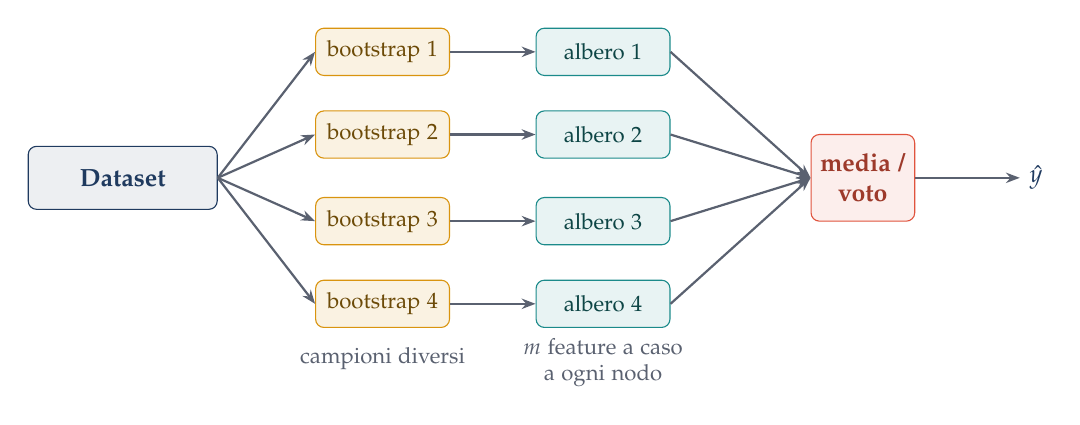
\begin{tikzpicture}[x=1cm,y=1cm,
  dato/.style={draw=navy,fill=navy!8,rounded corners=3pt,minimum width=2.4cm,minimum height=.8cm,font=\headfont\bfseries\small,text=navy},
  boot/.style={draw=ambra,fill=ambra!12,rounded corners=3pt,minimum width=1.7cm,minimum height=.6cm,font=\headfont\footnotesize,text=ambra!50!black},
  alb/.style={draw=teal,fill=teal!10,rounded corners=3pt,minimum width=1.7cm,minimum height=.6cm,font=\headfont\footnotesize,text=teal!50!black},
  frec/.style={-{Stealth[length=5pt]},line width=.8pt,color=grigio}]
  \node[dato] (D) at (0,0) {Dataset};
  \foreach \i/\y in {1/1.6,2/.55,3/-.55,4/-1.6}{
    \node[boot] (b\i) at (3.3,\y) {bootstrap \i};
    \node[alb] (t\i) at (6.1,\y) {albero \i};
    \draw[frec] (D.east) -- (b\i.west);
    \draw[frec] (b\i) -- (t\i);}
  \node[font=\headfont\footnotesize,text=grigio] at (3.3,-2.3) {campioni diversi};
  \node[font=\headfont\footnotesize,text=grigio,align=center] at (6.1,-2.35) {$m$ feature a caso\\a ogni nodo};
  \node[draw=rosso,fill=rosso!10,rounded corners=3pt,minimum height=1.1cm,font=\headfont\bfseries\small,text=rosso!70!black,align=center] (V) at (9.4,0) {media /\\voto};
  \foreach \i in {1,...,4}{\draw[frec] (t\i.east) -- (V.west);}
  \node[font=\headfont\bfseries\small,text=navy] (P) at (11.6,0) {$\hat y$};
  \draw[frec] (V) -- (P);
\end{tikzpicture}
\end{center}
\didascalia{Schema generale: dallo stesso dataset si generano $B$ campioni bootstrap, si addestra un albero «randomizzato» su ciascuno e si combinano le risposte.}

\subsection{Perché la media aiuta: anticipo del risultato chiave}

Se $B$ alberi hanno ciascuno varianza $\sigma^2$ e tra due alberi qualunque la correlazione è $\rho$, la varianza della loro media è (lo dimostreremo nel capitolo 4)
\begin{formula}
$\displaystyle \Var\!\Big(\frac1B\sum_{b=1}^{B}T_b\Big)=\rho\,\sigma^2+\frac{1-\rho}{B}\,\sigma^2 .$
\end{formula}
Il secondo termine sparisce aggiungendo alberi; il primo no. Per questo \hl{non basta avere molti alberi: bisogna che siano poco correlati}. Il bootstrap e la scelta casuale delle feature servono esattamente a ridurre $\rho$.

\begin{mlbox}[Nel mondo reale]
Il Random Forest è tra i modelli più usati su \key{dati tabellari} (righe = esempi, colonne = variabili): diagnostica medica, rischio di credito, previsione della domanda, telerilevamento, bioinformatica. Funziona bene «così com'è», con pochi parametri da regolare, e per questo è spesso il primo modello robusto da provare dopo una regressione lineare o logistica.
\end{mlbox}

\begin{appunti}{Riepilogo del capitolo}
\begin{itemize}
  \item Random Forest = \hl{molti alberi di decisione} + \hl{media} delle risposte.
  \item Gli alberi singoli hanno basso bias ma alta varianza; la media riduce la varianza.
  \item La media funziona solo se gli alberi sono \key{diversi}: bootstrap dei dati + $m$ feature casuali a ogni nodo.
  \item Varianza della media: $\rho\sigma^2+(1-\rho)\sigma^2/B$ $\Rightarrow$ conta ridurre la correlazione $\rho$.
\end{itemize}
\end{appunti}

\sezione{2}{Il mattone: l'albero di decisione}{Parte I · CART, impurità e scelta degli split}

\begin{inbreve}
Un albero di decisione divide lo spazio delle feature in rettangoli con domande del tipo $x_j\le t$. A ogni nodo sceglie la coppia (feature $j$, soglia $t$) che rende i due figli \hl{più «puri»} possibile, misurando la purezza con l'indice di \key{Gini}, l'\key{entropia} o l'\key{errore quadratico}. scikit-learn usa una versione ottimizzata dell'algoritmo \hl{CART}.
\end{inbreve}

\subsection{Come ragiona un albero}

\begin{intuizione}[Il gioco delle 20 domande]
Pensa al gioco «indovina chi»: a ogni turno scegli la domanda che \hl{elimina più incertezza}. «È un uomo?» divide i candidati a metà; «ha il cappello rosso?» ne elimina uno solo. L'albero fa lo stesso: tra tutte le domande possibili sceglie quella che separa meglio le classi, poi ripete il gioco separatamente su ciascuno dei due gruppi ottenuti.
\end{intuizione}

\begin{center}
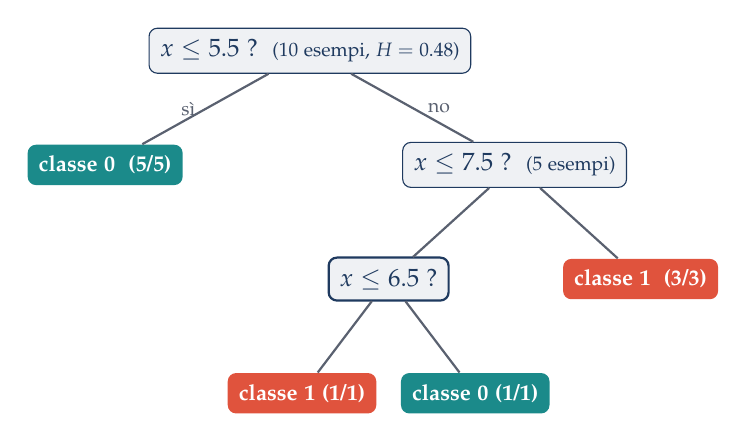
\begin{tikzpicture}[level distance=1.45cm,
  level 1/.style={sibling distance=5.2cm},level 2/.style={sibling distance=3.2cm},level 3/.style={sibling distance=2.2cm},
  nodo/.style={draw=navy,fill=navy!7,rounded corners=3pt,font=\headfont\small,text=navy,inner sep=4pt},
  foglia/.style={rounded corners=3pt,font=\headfont\bfseries\footnotesize,inner sep=4pt,text=white},
  edge from parent/.style={draw=grigio,line width=.8pt},
  every label/.style={font=\headfont\scriptsize,text=grigio}]
  \node[nodo] {$x\le 5.5$ ?\ \ {\scriptsize(10 esempi, $H=0.48$)}}
    child {node[foglia,fill=teal] {classe 0 \ (5/5)} edge from parent node[left,font=\headfont\scriptsize,text=grigio]{sì\ }}
    child {node[nodo] {$x\le 7.5$ ?\ \ {\scriptsize(5 esempi)}}
      child {node[nodo] {$x\le 6.5$ ?}
        child {node[foglia,fill=rosso] {classe 1 (1/1)}}
        child {node[foglia,fill=teal] {classe 0 (1/1)}}}
      child {node[foglia,fill=rosso] {classe 1 \ (3/3)}}
      edge from parent node[right,font=\headfont\scriptsize,text=grigio]{\ no}};
\end{tikzpicture}
\end{center}
\didascalia{L'albero completo ottenuto sull'esempio di questo capitolo (ore di studio $\rightarrow$ promosso/bocciato). L'ultimo split isola un singolo esempio «anomalo»: è il primo segnale di \emph{overfitting}.}

\subsection{La matematica dello split}

\begin{tecnica}[Formulazione CART (documentazione scikit-learn)]
Sia $Q_m$ l'insieme degli $n_m$ esempi che arrivano al nodo $m$. Un candidato split è $\theta=(j,t_m)$: feature $j$ e soglia $t_m$. Esso divide i dati in
\[
Q_m^{\mathrm{sx}}(\theta)=\{(\x,y)\,:\,x_j\le t_m\},\qquad Q_m^{\mathrm{dx}}(\theta)=Q_m\setminus Q_m^{\mathrm{sx}}(\theta).
\]
La qualità dello split è l'\hl{impurità pesata} dei figli:
\[
G(Q_m,\theta)=\frac{n_m^{\mathrm{sx}}}{n_m}\,H\big(Q_m^{\mathrm{sx}}(\theta)\big)+\frac{n_m^{\mathrm{dx}}}{n_m}\,H\big(Q_m^{\mathrm{dx}}(\theta)\big),
\qquad
\theta^*=\argmin_{\theta}\,G(Q_m,\theta).
\]
La ricerca è \key{golosa} (\emph{greedy}): per ogni feature si provano come soglie i punti medi tra valori consecutivi ordinati e si tiene il minimo. Poi si ripete ricorsivamente sui due figli, finché non si raggiunge un criterio di arresto (profondità massima, numero minimo di esempi, nodo puro).
\end{tecnica}

Le funzioni di impurità $H$ più usate, con $p_{mk}$ = frazione di esempi della classe $k$ nel nodo $m$:

\begin{center}
\renewcommand{\arraystretch}{1.55}
\rowcolors{2}{chiaro}{white}
\begin{tabularx}{\linewidth}{>{\headfont\bfseries\small}l >{\centering\arraybackslash}X >{\small}p{4.3cm}}
\rowcolor{navy}\thd{Criterio} & \thd{Formula} & \thd{In scikit-learn}\\
Gini & $H(Q_m)=\sum_k p_{mk}(1-p_{mk})=1-\sum_k p_{mk}^2$ & \texttt{criterion="gini"} (default classificazione)\\
Entropia & $H(Q_m)=-\sum_k p_{mk}\log p_{mk}$ & \texttt{"entropy"} / \texttt{"log\_loss"}\\
Errore quadratico & $H(Q_m)=\dfrac{1}{n_m}\sum_{y\in Q_m}(y-\bar y_m)^2$ & \texttt{"squared\_error"} (default regressione)\\
\end{tabularx}
\end{center}

\begin{intuizione}[Cosa misura il Gini]
L'indice di Gini è la \hl{probabilità di sbagliare} se prendi un esempio a caso dal nodo e gli assegni un'etichetta estratta a caso secondo le proporzioni del nodo. Nodo puro (tutti della stessa classe): $H=0$. Nodo 50/50 con due classi: $H=0.5$, il massimo.
\end{intuizione}

\begin{esempio}[Uno split calcolato a mano]
Dieci studenti, una sola feature $x$ = ore di studio, classe $1$ = promosso:
\begin{center}
\small
\begin{tabular}{c|cccccccccc}
$x$ & 1&2&3&4&5&6&7&8&9&10\\\hline
$y$ & 0&0&0&0&0&1&0&1&1&1
\end{tabular}
\end{center}
\textbf{Radice.} 4 promossi su 10: $H=1-(0.4^2+0.6^2)=1-0.52=\mathbf{0.48}$.

\textbf{Soglia $t=5.5$.} Sinistra $\{1,\dots,5\}$: tutti 0, $H_{\mathrm{sx}}=0$. Destra $\{6,\dots,10\}$: 4 promossi su 5, $H_{\mathrm{dx}}=1-(0.8^2+0.2^2)=0.32$.
\[
G(5.5)=\tfrac{5}{10}\cdot 0+\tfrac{5}{10}\cdot 0.32=\mathbf{0.16}.
\]
\textbf{Soglia $t=7.5$.} Sinistra: 7 esempi con 1 promosso, $H=1-\big((\tfrac17)^2+(\tfrac67)^2\big)\approx0.245$. Destra: 3 promossi su 3, $H=0$. $G(7.5)=\tfrac{7}{10}\cdot0.245\approx\mathbf{0.171}$.

Provando tutte le 9 soglie (figura sotto) il minimo è $G=0.16$ in $t^*=5.5$: è il primo split dell'albero. La \key{riduzione di impurità} è $0.48-0.16=0.32$.
\end{esempio}

\par\noindent\begin{minipage}{\linewidth}
\fig[.98\linewidth]{split.pdf}
\didascalia{A sinistra i dati con la soglia ottima. A destra $G(t)$ per tutte le soglie candidate: il minimo (in ambra) si trova in $t=5.5$. Valori ricalcolati in Python.}
\end{minipage}\par

\subsection{Il difetto: alta varianza}

Un albero cresciuto fino in fondo isola anche i punti rumorosi (come lo studente con 7 ore e bocciato). Sui dati di addestramento sbaglia zero volte, ma su dati nuovi generalizza male: è il classico \hl{overfitting}. Inoltre, poiché gli split sono scelti in modo goloso dall'alto verso il basso, \key{un piccolo cambiamento nei dati può cambiare il primo split} e quindi tutto l'albero sotto di esso.

\begin{attenzione}[Due rimedi diversi]
Ci sono due modi di combattere la varianza di un albero:
\begin{itemize}
  \item \hl{potarlo o limitarlo} (\texttt{max\_depth}, \texttt{min\_samples\_leaf}, \texttt{ccp\_alpha}): riduce la varianza ma \emph{aumenta il bias};
  \item \hl{farne la media con altri alberi} diversi: riduce la varianza lasciando il bias quasi invariato. È la strada del Random Forest, che per questo usa di default alberi \key{non potati}.
\end{itemize}
\end{attenzione}

\begin{appunti}{Riepilogo del capitolo}
\begin{itemize}
  \item Un albero divide lo spazio con domande $x_j\le t$; ogni foglia dà una previsione costante.
  \item Split ottimo: $\theta^*=\argmin_\theta G(Q_m,\theta)$, con $G$ = media pesata delle impurità dei figli.
  \item Impurità: Gini $1-\sum_k p_k^2$, entropia $-\sum_k p_k\log p_k$, errore quadratico per la regressione.
  \item Albero profondo = basso bias ma \hl{alta varianza}: è il mattone perfetto da mettere in media.
\end{itemize}
\end{appunti}

\sezione{3}{Bootstrap e bagging}{Parte I · prima fonte di casualità e stima out-of-bag}

\begin{inbreve}
Il \hl{bagging} (\emph{bootstrap aggregating}, Breiman 1996) addestra lo stesso modello su $B$ campioni \key{bootstrap} del dataset e ne fa la media. Ogni campione contiene in media il \hl{63{,}2\%} degli esempi distinti; il restante 36{,}8\% sono gli esempi \key{out-of-bag} (OOB), che forniscono una stima gratuita dell'errore di generalizzazione.
\end{inbreve}

\subsection{Il campione bootstrap}

\begin{intuizione}[Pescare dall'urna rimettendo dentro]
Metti i nomi di tutti gli $n$ esempi in un'urna. Peschi un nome, lo scrivi, \hl{lo rimetti nell'urna}, e ripeti $n$ volte. Ottieni un nuovo dataset della stessa dimensione, in cui alcuni esempi compaiono più volte e altri mai. Ogni albero vede così un «mondo» leggermente diverso, e per questo cresce in modo diverso.
\end{intuizione}

\begin{tecnica}[Quanti esempi distinti finiscono in un bootstrap?]
La probabilità che un dato esempio \emph{non} venga scelto in una estrazione è $1-\frac1n$; in $n$ estrazioni indipendenti è $\left(1-\frac1n\right)^n$. Quindi
\[
P(\text{esempio incluso})=1-\Big(1-\frac1n\Big)^{n}\ \xrightarrow[n\to\infty]{}\ 1-\frac1e\approx 0.632 .
\]
In media ogni albero vede circa il \hl{63{,}2\%} degli esempi distinti; il restante \hl{36{,}8\%} è \key{out-of-bag} per quell'albero.
\end{tecnica}

\par\noindent\begin{minipage}{\linewidth}
\fig[.8\linewidth]{bootstrap.pdf}
\didascalia{La frazione di esempi distinti in un campione bootstrap converge rapidamente a $1-1/e$. Già con $n=100$ vale $0.634$; con $n=1000$ vale $0.6323$.}
\end{minipage}\par

\subsection{Bagging: mettere in media}

\begin{tecnica}[Definizione]
Dati i campioni bootstrap $\mathcal{Z}^{*1},\dots,\mathcal{Z}^{*B}$ e il modello $\hat f^{*b}$ addestrato su $\mathcal{Z}^{*b}$:
\begin{align*}
\hat f_{\mathrm{bag}}(\x)&=\frac1B\sum_{b=1}^{B}\hat f^{*b}(\x) &&\text{(regressione)},\\
\hat C_{\mathrm{bag}}(\x)&=\argmax_k\ \frac1B\sum_{b=1}^{B}\hat p^{*b}_k(\x) &&\text{(classificazione)}.
\end{align*}
Il bagging riduce la varianza di modelli instabili come gli alberi, lasciando il loro bias sostanzialmente invariato: il valore atteso della media di $B$ alberi identicamente distribuiti è uguale al valore atteso di un singolo albero.
\end{tecnica}

\subsection{La stima out-of-bag (OOB)}

Ogni esempio $i$ è OOB per circa un terzo degli alberi. Possiamo quindi \hl{prevedere $y_i$ usando solo gli alberi che non l'hanno mai visto} e confrontare con il valore vero: è come una validazione incrociata, ma ottenuta gratis durante l'addestramento.

\begin{tecnica}[Errore OOB]
Sia $\mathcal{B}_i=\{b:\ i\notin\mathcal{Z}^{*b}\}$ l'insieme degli alberi per cui l'esempio $i$ è out-of-bag. La previsione OOB è
\[
\hat f^{\mathrm{oob}}(\x_i)=\frac{1}{|\mathcal{B}_i|}\sum_{b\in\mathcal{B}_i}\hat f^{*b}(\x_i),
\qquad
\mathrm{Err}_{\mathrm{oob}}=\frac1n\sum_{i=1}^{n}L\big(y_i,\hat f^{\mathrm{oob}}(\x_i)\big).
\]
In scikit-learn si attiva con \texttt{oob\_score=True}: il punteggio (accuratezza per i classificatori, $R^2$ per i regressori, oppure una funzione a scelta) è in \texttt{oob\_score\_}, le previsioni OOB in \texttt{oob\_decision\_function\_} (classificazione) o \texttt{oob\_prediction\_} (regressione).
\end{tecnica}

\begin{attenzione}[Quando l'OOB non basta]
\begin{itemize}
  \item Con \hl{pochi alberi} alcuni esempi non sono mai OOB: la loro previsione non esiste e scikit-learn può restituire \texttt{NaN} in \texttt{oob\_decision\_function\_} (con un avviso). Usa abbastanza alberi.
  \item L'OOB funziona solo con \texttt{bootstrap=True} (il default).
  \item Se fai tuning degli iperparametri guardando l'OOB, la stima diventa ottimistica: per la valutazione finale tieni comunque un \key{test set} mai usato.
\end{itemize}
\end{attenzione}

\begin{esempio}[Un mini bootstrap]
Dataset con $n=6$ esempi $\{1,2,3,4,5,6\}$. Un'estrazione con reinserimento può dare $\{2,2,5,1,5,6\}$: gli esempi distinti sono $\{1,2,5,6\}$, cioè 4 su 6 ($\approx 67\%$), e gli OOB sono $\{3,4\}$. Per $n=6$ la teoria prevede in media $1-(5/6)^6\approx 0.665$ esempi distinti.
\end{esempio}

\begin{appunti}{Riepilogo del capitolo}
\begin{itemize}
  \item Bootstrap = $n$ estrazioni \hl{con reinserimento}; include in media $1-1/e\approx63{,}2\%$ degli esempi.
  \item Bagging = media dei modelli addestrati sui bootstrap: riduce la varianza, non il bias.
  \item Errore OOB = stima dell'errore usando per ogni esempio solo gli alberi che non l'hanno visto.
  \item In scikit-learn: \texttt{bootstrap=True}, \texttt{oob\_score=True}, attributo \texttt{oob\_score\_}.
\end{itemize}
\end{appunti}

\sezione{4}{Il Random Forest}{Parte I · decorrelare gli alberi, algoritmo e teoria}

\begin{inbreve}
Il Random Forest è un bagging di alberi con un'aggiunta: a ogni nodo lo split viene cercato solo tra \hl{$m$ feature estratte a caso} tra le $p$ disponibili. Questo \key{decorrela} gli alberi e rende la media molto più efficace. La teoria di Breiman mostra che l'errore dipende da due quantità: la \hl{forza} dei singoli alberi e la loro \hl{correlazione}.
\end{inbreve}

\subsection{Perché il bagging da solo non basta}

\begin{intuizione}[Tutti seguono la stessa star]
Supponi che nel dataset ci sia una variabile molto forte. Con il solo bagging, quasi tutti gli alberi la useranno nel primo split, e poi in modo simile nei successivi: gli alberi si \hl{assomigliano} e i loro errori vanno nella stessa direzione. È la folla che copia il vicino. Se invece a ogni nodo un albero può guardare solo alcune variabili a caso, a volte la «star» non è disponibile e l'albero deve trovare altre strade: gli alberi diventano più diversi e la media funziona meglio.
\end{intuizione}

\begin{tecnica}[Varianza della media di variabili correlate]
Siano $T_1,\dots,T_B$ identicamente distribuite con $\Var(T_b)=\sigma^2$ e correlazione $\rho$ per ogni coppia ($\mathrm{Cov}(T_b,T_c)=\rho\sigma^2$ per $b\ne c$). Allora
\[
\Var\!\Big(\frac1B\sum_{b}T_b\Big)=\frac{1}{B^2}\Big[\underbrace{B\sigma^2}_{\text{varianze}}+\underbrace{B(B-1)\rho\sigma^2}_{\text{covarianze}}\Big]
=\rho\sigma^2+\frac{1-\rho}{B}\sigma^2 .
\]
Per $B\to\infty$ la varianza scende fino a $\rho\sigma^2$ e non oltre. Il Random Forest riduce $\rho$ scegliendo a caso le feature candidate a ogni split (\emph{The Elements of Statistical Learning}, §15.2).
\end{tecnica}

\par\noindent\begin{minipage}{\linewidth}
\fig[.8\linewidth]{varianza.pdf}
\didascalia{Varianza della media (in unità di $\sigma^2$) al crescere del numero di alberi $B$. Ogni curva si appiattisce sul proprio $\rho$ (linee tratteggiate): con alberi molto correlati, aggiungerne altri serve a poco.}
\end{minipage}\par

\subsection{L'algoritmo}

\begin{tecnica}[Random Forest per regressione o classificazione (ESL, Algoritmo 15.1)]
\textbf{Addestramento.} Per $b=1,\dots,B$:
\begin{passi}
  \item estrai un campione bootstrap $\mathcal{Z}^{*b}$ di dimensione $n$ dai dati;
  \item fai crescere un albero $T_b$ su $\mathcal{Z}^{*b}$ ripetendo, a ogni nodo, finché il nodo ha almeno $n_{\min}$ esempi:
    \begin{itemize}
      \item scegli a caso $m$ feature tra le $p$;
      \item trova lo split migliore solo tra queste $m$ (criterio del capitolo 2);
      \item dividi il nodo in due figli.
    \end{itemize}
\end{passi}
\textbf{Previsione} per un nuovo $\x$:
\begin{align*}
\hat f_{\mathrm{rf}}^{B}(\x)&=\frac1B\sum_{b=1}^{B}T_b(\x) &&\text{(regressione)},\\
\hat C_{\mathrm{rf}}^{B}(\x)&=\text{voto di maggioranza}\ \big\{\hat C_b(\x)\big\}_{b=1}^{B} &&\text{(classificazione)}.
\end{align*}
Valori consigliati in letteratura: $m=\lfloor\sqrt p\rfloor$ e $n_{\min}=1$ per la classificazione; $m=\lfloor p/3\rfloor$ e $n_{\min}=5$ per la regressione.
\end{tecnica}

\begin{attenzione}[Voto oppure media delle probabilità?]
Breiman (2001) combina gli alberi con un \hl{voto di maggioranza}. scikit-learn invece \hl{fa la media delle probabilità} stimate dai singoli alberi e sceglie la classe con probabilità media più alta («invece di lasciare che ogni classificatore voti per una sola classe», dice la documentazione). Le due regole quasi sempre coincidono, ma non sempre: ricordalo se confronti implementazioni diverse.
\end{attenzione}

\subsection{La teoria di Breiman: forza e correlazione}

\begin{tecnica}[Margine, forza, correlazione (Breiman 2001)]
Per un insieme di classificatori $h_1,\dots,h_K$ il \key{margine} di un esempio $(\x,y)$ è
\[
mg(\x,y)=\operatorname{av}_k\,I\big(h_k(\x)=y\big)-\max_{j\ne y}\ \operatorname{av}_k\,I\big(h_k(\x)=j\big),
\]
cioè di quanto la frazione di voti per la classe giusta supera quella della classe sbagliata più votata. Se $mg<0$ l'esempio è classificato male. Breiman dimostra che:
\begin{itemize}
  \item al crescere del numero di alberi l'errore di generalizzazione \hl{converge quasi certamente} a un limite: \key{aggiungere alberi non causa overfitting};
  \item detta $s$ la \hl{forza} (margine atteso dei singoli alberi) e $\bar\rho$ la \hl{correlazione} media tra alberi, vale il limite superiore
\end{itemize}
\[
PE^*\ \le\ \frac{\bar\rho\,(1-s^2)}{s^2}.
\]
Per ridurre l'errore servono \hl{alberi forti} ($s$ grande) e \hl{poco correlati} ($\bar\rho$ piccolo).
\end{tecnica}

\begin{intuizione}[Il compromesso su $m$]
Il parametro $m$ regola proprio questo compromesso. Con $m$ piccolo gli alberi sono molto diversi ($\bar\rho$ scende) ma ciascuno è più debole ($s$ scende). Con $m=p$ ogni albero è il più forte possibile, ma tutti si assomigliano: è il semplice bagging. Il valore migliore sta nel mezzo e \key{dipende dai dati}: per questo $m$ (\texttt{max\_features}) è uno dei due parametri principali da regolare.
\end{intuizione}

\subsection{Cosa cambia nei confini di decisione}

\par\noindent\begin{minipage}{\linewidth}
\fig[\linewidth]{confini.pdf}
\didascalia{Dataset «due lune» con rumore. Un albero profondo disegna confini a scalini che inseguono il rumore; un albero su un altro bootstrap ne disegna di diversi (alta varianza). La foresta (sfumature = probabilità media) produce un confine molto più regolare.}
\end{minipage}\par

\begin{mlbox}[Bias e varianza in una frase]
Gli alberi del Random Forest hanno lo stesso valore atteso di un singolo albero randomizzato, quindi il bias della foresta è circa quello di un albero; il guadagno arriva tutto dalla \hl{riduzione della varianza}. La documentazione di scikit-learn precisa che le due fonti di casualità riducono la varianza «a volte al costo di un leggero aumento del bias»: ogni albero, vedendo meno dati e meno feature, è un po' meno preciso.
\end{mlbox}

\begin{appunti}{Riepilogo del capitolo}
\begin{itemize}
  \item Random Forest = bagging di alberi + \hl{$m$ feature casuali a ogni nodo}.
  \item $\Var(\text{media})=\rho\sigma^2+(1-\rho)\sigma^2/B$: la casualità sulle feature abbassa $\rho$.
  \item Previsione: media (regressione); voto (Breiman) o media delle probabilità (scikit-learn).
  \item Breiman: più alberi non portano overfitting; $PE^*\le\bar\rho(1-s^2)/s^2$.
  \item Default classici: $m=\sqrt p$ (classificazione), $m=p/3$ (regressione).
\end{itemize}
\end{appunti}

\sezione{5}{Gli iperparametri}{Parte I · cosa regolare e cosa lasciare ai default}

\begin{inbreve}
Il Random Forest funziona bene anche con i valori predefiniti. I due parametri che contano di più, secondo la documentazione di scikit-learn, sono \hl{\texttt{n\_estimators}} (quanti alberi) e \hl{\texttt{max\_features}} (quante feature candidate a ogni split). Gli altri controllano quanto cresce ogni albero, la casualità e le risorse di calcolo.
\end{inbreve}

\begin{attenzione}[Le fonti non concordano su $m$ in regressione]
Il valore «classico» per la regressione, proposto da Breiman e riportato in \emph{The Elements of Statistical Learning}, è $m=p/3$. In scikit-learn invece il default di \texttt{RandomForestRegressor} è \hl{\texttt{max\_features=1.0}}, cioè \key{tutte le feature}: senza modifiche ottieni un bagging di alberi, non un Random Forest «alla Breiman». La documentazione lo dice esplicitamente e indica \texttt{max\_features=1.0} come scelta empirica ragionevole. Se vuoi la regola classica scrivi \texttt{max\_features=1/3} (come nell'esempio 3).
\end{attenzione}

\begin{attenzione}[Tutorial vecchi]
Alcuni default sono cambiati nel tempo: \texttt{n\_estimators} è passato da 10 a 100 nella versione 0.22; \texttt{max\_features="auto"} è stato eliminato dalla versione 1.3 (prima per i classificatori equivaleva a \texttt{"sqrt"}). Codice trovato online con \texttt{"auto"} oggi dà errore.
\end{attenzione}

\subsection{Mappa dei parametri principali}

\begin{center}
\small
\renewcommand{\arraystretch}{1.35}\renewcommand\tabularxcolumn[1]{m{#1}}
\rowcolors{2}{chiaro}{white}
\begin{tabularx}{\linewidth}{>{\leavevmode\ttfamily\color{navy}}m{3.25cm} >{\centering\arraybackslash}m{2.65cm} >{\raggedright\arraybackslash}X}
\rowcolor{navy}\thd{Parametro} & \thd{Default} & \thd{Significato e effetto}\\
n\_estimators & 100 & Numero di alberi $B$. Più alberi = stima più stabile, mai overfitting, ma più tempo e memoria.\\
max\_features & \texttt{"sqrt"} (clf) \newline \texttt{1.0} (reg) & $m$, feature candidate a ogni nodo. Intero, frazione di $p$, \texttt{"sqrt"}, \texttt{"log2"} o \texttt{None} ($=p$). Più basso = alberi più diversi ma più deboli.\\
max\_depth & \texttt{None} & Profondità massima. \texttt{None} = cresce finché le foglie sono pure o troppo piccole.\\
min\_samples\_split & 2 & Esempi minimi in un nodo per poterlo dividere.\\
min\_samples\_leaf & 1 & Esempi minimi in ogni foglia: valori 3--10 «lisciano» il modello, soprattutto in regressione.\\
max\_leaf\_nodes & \texttt{None} & Numero massimo di foglie per albero.\\
\end{tabularx}
\end{center}
\begin{center}
\small
\renewcommand{\arraystretch}{1.35}\renewcommand\tabularxcolumn[1]{m{#1}}
\rowcolors{2}{chiaro}{white}
\begin{tabularx}{\linewidth}{>{\leavevmode\ttfamily\color{navy}}m{3.25cm} >{\centering\arraybackslash}m{2.65cm} >{\raggedright\arraybackslash}X}
\rowcolor{navy}\thd{Parametro} & \thd{Default} & \thd{Significato e effetto}\\
criterion & \texttt{"gini"} / \newline\texttt{"squared\_error"} & Funzione di impurità (capitolo 2).\\
bootstrap & \texttt{True} & Se \texttt{False}, ogni albero usa tutto il dataset (resta solo la casualità sulle feature).\\
max\_samples & \texttt{None} & Dimensione del bootstrap (intero o frazione di $n$).\\
oob\_score & \texttt{False} & Calcola la stima out-of-bag (capitolo 3).\\
class\_weight & \texttt{None} & Pesi delle classi; \texttt{"balanced"} o \texttt{"balanced\_subsample"} per classi sbilanciate.\\
n\_jobs & \texttt{None} & Core usati; \texttt{-1} = tutti. Gli alberi si addestrano in parallelo.\\
random\_state & \texttt{None} & Seme: fissalo per avere risultati riproducibili.\\
warm\_start & \texttt{False} & Se \texttt{True}, una nuova \texttt{fit} aggiunge alberi a quelli esistenti.\\
ccp\_alpha & 0.0 & Potatura costo-complessità dei singoli alberi.\\
\end{tabularx}
\end{center}
\didascalia{Firma di \texttt{RandomForestClassifier} / \texttt{RandomForestRegressor} in scikit-learn 1.9 (valori verificati sulla documentazione ufficiale).}

\subsection{Quanti alberi servono?}

\par\noindent\begin{minipage}{\linewidth}
\fig[.8\linewidth]{oob.pdf}
\didascalia{Errore OOB sul dataset Breast Cancer al crescere di \texttt{n\_estimators}, con tre valori di \texttt{max\_features} (codice in \texttt{figs.py}, con \texttt{warm\_start=True}). L'errore oscilla molto con pochi alberi e poi si stabilizza intorno a 3{,}4--3{,}5\%: oltre qualche centinaio di alberi il guadagno è trascurabile.}
\end{minipage}\par

\begin{intuizione}[Come leggere il grafico]
Aggiungere alberi \hl{non peggiora mai} l'errore atteso (risultato di Breiman), ma dopo un certo punto non lo migliora più: costa solo tempo. Su questo dataset le tre scelte di \texttt{max\_features} finiscono quasi alla pari; su altri dati le differenze possono essere grandi. È il motivo per cui $m$ si \key{sceglie con la validazione}, non a priori.
\end{intuizione}

\subsection{Strategia di tuning consigliata}

\begin{passi}
  \item Parti dai default, con \texttt{n\_estimators} tra 300 e 500 e \texttt{random\_state} fissato.
  \item Regola \texttt{max\_features}: prova ad esempio \texttt{"sqrt"}, \texttt{0.3}, \texttt{0.5}, \texttt{1.0}.
  \item Regola la crescita degli alberi con \texttt{min\_samples\_leaf} (1, 3, 5, 10) o \texttt{max\_depth}.
  \item Usa la \key{validazione incrociata} (\texttt{GridSearchCV} o \texttt{RandomizedSearchCV}, capitolo 9) o, per un controllo veloce, l'OOB.
  \item Valuta il modello finale una sola volta sul test set.
\end{passi}

\begin{consiglio}[Memoria e tempi]
Con i default gli alberi crescono completamente: la dimensione del modello è dell'ordine di $O(M\cdot N\log N)$ nodi, con $M$ alberi ed $N$ esempi, e su dataset grandi può occupare molta RAM. Se il file salvato è troppo grande, aumenta \texttt{min\_samples\_leaf}, imposta \texttt{max\_depth} o \texttt{max\_leaf\_nodes}. \texttt{n\_jobs=-1} usa tutti i core, ma l'accelerazione non è lineare.
\end{consiglio}

\begin{appunti}{Riepilogo del capitolo}
\begin{itemize}
  \item Parametri principali: \hl{\texttt{n\_estimators}} e \hl{\texttt{max\_features}}.
  \item Default sklearn: \texttt{"sqrt"} in classificazione, \texttt{1.0} (tutte) in regressione.
  \item Complessità del singolo albero: \texttt{max\_depth}, \texttt{min\_samples\_leaf}, \texttt{min\_samples\_split}, \texttt{max\_leaf\_nodes}.
  \item Più alberi non danno overfitting; oltre qualche centinaio il guadagno è minimo.
  \item Scegli gli iperparametri con validazione incrociata; test set solo alla fine.
\end{itemize}
\end{appunti}

\sezione{6}{Importanza delle feature}{Parte I · MDI e importanza per permutazione}

\begin{inbreve}
Un Random Forest non ha coefficienti come una regressione, ma può dire \hl{quanto conta ogni variabile}. Ci sono due misure: la \key{MDI} (diminuzione media di impurità, \texttt{feature\_importances\_}), veloce ma distorta, e l'\key{importanza per permutazione}, più affidabile, calcolata su dati non usati per l'addestramento.
\end{inbreve}

\subsection{MDI: Mean Decrease in Impurity}

\begin{tecnica}[Definizione]
Ogni volta che un nodo $t$ viene diviso sulla feature $j$, l'impurità cala di
\[
\Delta i(t)=\frac{n_t}{n}\Big[H(t)-\frac{n_{t}^{\mathrm{sx}}}{n_t}H(t^{\mathrm{sx}})-\frac{n_t^{\mathrm{dx}}}{n_t}H(t^{\mathrm{dx}})\Big].
\]
L'importanza MDI della feature $j$ somma questi cali su tutti i nodi che usano $j$ e ne fa la media sugli alberi:
\[
\mathrm{MDI}(j)=\frac1B\sum_{b=1}^{B}\ \sum_{t\in T_b:\ v(t)=j}\Delta i(t),
\]
poi le importanze vengono normalizzate in modo da sommare a 1. In scikit-learn è l'attributo \texttt{feature\_importances\_}.
\end{tecnica}

\begin{attenzione}[I due difetti della MDI]
La documentazione di scikit-learn segnala che la MDI:
\begin{itemize}
  \item è calcolata sui \hl{dati di addestramento}, quindi può dare importanza a feature che servono solo a memorizzare il rumore;
  \item è \hl{distorta verso le feature con molti valori distinti} (alta cardinalità, ad esempio un identificativo numerico), che offrono più soglie candidate.
\end{itemize}
Per conclusioni affidabili usa l'importanza per permutazione.
\end{attenzione}

\subsection{Importanza per permutazione}

\begin{intuizione}[Mescola una colonna e guarda cosa succede]
Prendi il modello già addestrato e un set di dati di validazione. Mescola a caso \hl{solo la colonna $j$}, lasciando invariate le altre: il legame tra quella variabile e il target è distrutto. Se il punteggio del modello crolla, la variabile era importante; se non cambia, il modello non la usava (o poteva farne a meno).
\end{intuizione}

\begin{tecnica}[Definizione (sklearn.inspection)]
Sia $s$ il punteggio del modello sui dati di riferimento $D$. Per ogni feature $j$ e per ogni ripetizione $k=1,\dots,K$ si permuta la colonna $j$ ottenendo $\tilde D_{k,j}$ e si calcola il punteggio $s_{k,j}$. L'importanza è
\[
i_j=s-\frac{1}{K}\sum_{k=1}^{K}s_{k,j}.
\]
Si calcola con \texttt{permutation\_importance(modello, X, y, n\_repeats=K, scoring=...)}; il risultato contiene \texttt{importances\_mean} e \texttt{importances\_std}. Funziona con qualsiasi modello, non solo con le foreste.
\end{tecnica}

\par\noindent\begin{minipage}{\linewidth}
\fig[\linewidth]{importanze.pdf}
\didascalia{Le 8 feature più importanti secondo la MDI nel modello dell'esempio 2 (Breast Cancer), confrontate con l'importanza per permutazione sul test set (AUC, 20 ripetizioni). Valori reali dall'esecuzione.}
\end{minipage}\par

\begin{esempio}[Cosa ci dice il confronto]
Le due misure concordano sulle feature in cima (\texttt{worst area}, \texttt{worst perimeter}, \texttt{worst concave points}), ma la permutazione dà valori \hl{molto piccoli}: mescolare \texttt{worst area} fa calare l'AUC solo di circa $0.004$. Il motivo è che in questo dataset molte feature sono \key{fortemente correlate} (raggio, perimetro e area misurano quasi la stessa cosa): se ne mescoli una, il modello usa le altre e quasi non se ne accorge.
\end{esempio}

\begin{attenzione}[Feature correlate]
Con feature correlate l'importanza per permutazione \hl{sottostima} ciascuna di esse, e la MDI divide il merito tra loro in modo arbitrario. Nessuna delle due misure dice che una variabile «causa» il target. Una soluzione suggerita dalla documentazione di scikit-learn è raggruppare le feature correlate (ad esempio con un clustering gerarchico sulle correlazioni) e tenerne una per gruppo.
\end{attenzione}

\begin{consiglio}[Quale usare]
Per un'occhiata veloce va bene \texttt{feature\_importances\_}. Per una relazione, una tesi o una decisione usa \texttt{permutation\_importance} su un \key{set di validazione o test}, riportando media e deviazione standard.
\end{consiglio}

\begin{appunti}{Riepilogo del capitolo}
\begin{itemize}
  \item MDI = somma dei cali di impurità dovuti alla feature, media sugli alberi, normalizzata a 1.
  \item MDI: veloce, ma calcolata sul training e distorta verso feature ad alta cardinalità.
  \item Permutazione: $i_j=s-\frac1K\sum_k s_{k,j}$, su dati non visti; più affidabile.
  \item Feature correlate: entrambe le misure vanno interpretate con cautela; importanza $\ne$ causalità.
\end{itemize}
\end{appunti}

\sezione{7}{Librerie e struttura del codice}{Parte II · gli strumenti Python e come organizzarli}

\begin{inbreve}
In Python il Random Forest si usa quasi sempre tramite \hl{scikit-learn}, affiancata da \key{NumPy} e \key{pandas} per i dati, \key{matplotlib} per i grafici e \key{joblib} per salvare il modello. Il codice segue sempre lo stesso schema: \hl{dati $\rightarrow$ suddivisione $\rightarrow$ pipeline $\rightarrow$ validazione e tuning $\rightarrow$ valutazione finale $\rightarrow$ salvataggio}.
\end{inbreve}

\subsection{Le librerie e a cosa servono}

\begin{center}
\small
\renewcommand{\arraystretch}{1.35}
\rowcolors{2}{chiaro}{white}
\begin{tabularx}{\linewidth}{>{\leavevmode\ttfamily\bfseries\color{navy}\footnotesize}p{3.7cm} X >{\ttfamily\footnotesize}p{4.2cm}}
\rowcolor{navy}\thd{Libreria / modulo} & \thd{A cosa serve} & \thd{Oggetti tipici}\\
numpy & Array numerici e calcolo vettoriale & array, random\\
pandas & Tabelle con nomi di colonna (\texttt{DataFrame}), lettura CSV/Excel & read\_csv, DataFrame\\
sklearn.ensemble & I modelli Random Forest & RandomForestClassifier, RandomForestRegressor\\
sklearn.model\_selection & Suddivisione dati, validazione incrociata, tuning & train\_test\_split, StratifiedKFold, GridSearchCV\\
sklearn.pipeline & Concatenare preprocessing e modello & Pipeline\\
sklearn.compose & Trattare colonne diverse in modo diverso & ColumnTransformer\\
sklearn.preprocessing \newline sklearn.impute & Codifica delle categorie, valori mancanti & OneHotEncoder, SimpleImputer\\
sklearn.metrics & Misure di qualità & accuracy\_score, roc\_auc\_score, r2\_score\\
sklearn.inspection & Interpretazione & permutation\_importance\\
matplotlib & Grafici & pyplot\\
joblib & Salvare e ricaricare modelli & dump, load\\
\end{tabularx}
\end{center}

\begin{terminale}{installazione}
§$§ python -m pip install scikit-learn pandas matplotlib joblib
§$§ python -c "import sklearn; print(sklearn.__version__)"
1.9.1
\end{terminale}

\subsection{L'interfaccia comune: \texttt{fit}, \texttt{predict}, \texttt{predict\_proba}}

\begin{intuizione}[Tutti i modelli parlano la stessa lingua]
In scikit-learn ogni modello è un oggetto \key{stimatore} con gli stessi metodi. Una volta imparato il Random Forest, sai già usare la regressione logistica, le SVM o il gradient boosting: cambia solo la riga in cui crei il modello.
\end{intuizione}

\begin{center}
\small
\renewcommand{\arraystretch}{1.35}
\rowcolors{2}{chiaro}{white}
\begin{tabularx}{\linewidth}{>{\leavevmode\ttfamily\color{navy}\footnotesize}p{4.6cm} X}
\rowcolor{navy}\thd{Metodo / attributo} & \thd{Cosa fa}\\
modello.fit(X, y) & Addestra il modello. Restituisce il modello stesso.\\
modello.predict(X) & Classe prevista (o valore, in regressione).\\
modello.predict\_proba(X) & Probabilità di ogni classe: media delle probabilità degli alberi.\\
modello.score(X, y) & Accuratezza (classificazione) o $R^2$ (regressione).\\
modello.estimators\_ & Lista degli alberi addestrati (oggetti \texttt{DecisionTree...}).\\
modello.classes\_ & Etichette delle classi, nell'ordine delle colonne di \texttt{predict\_proba}.\\
modello.feature\_importances\_ & Importanza MDI (capitolo 6).\\
modello.oob\_score\_ & Punteggio out-of-bag (se \texttt{oob\_score=True}).\\
\end{tabularx}
\end{center}
\didascalia{Per convenzione gli attributi che finiscono con «\texttt{\_}» esistono solo dopo \texttt{fit}.}

\subsection{Lo schema di un progetto}

\begin{center}
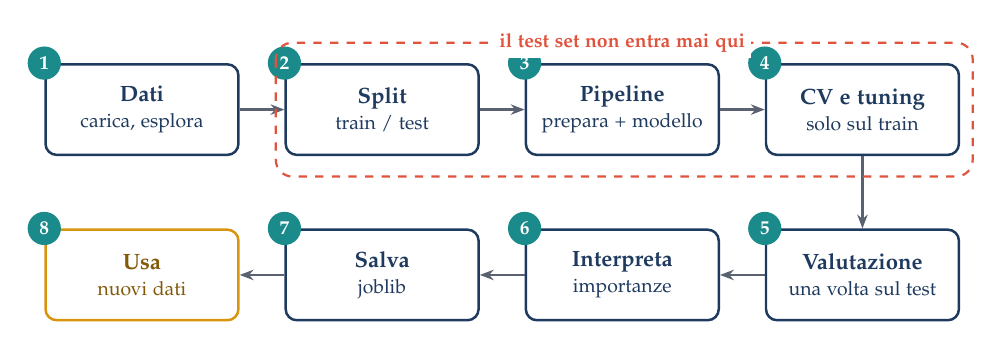
\begin{tikzpicture}[x=1cm,y=1cm,
  st/.style={draw=navy,fill=white,line width=.9pt,rounded corners=4pt,minimum width=2.45cm,minimum height=1.15cm,align=center,font=\headfont\footnotesize,text=navy},
  num/.style={circle,fill=teal,text=white,font=\headfont\bfseries\scriptsize,inner sep=1.5pt,minimum size=1.2em},
  fr/.style={-{Stealth[length=5pt]},line width=.9pt,color=grigio}]
  \node[st] (a) at (0,0) {\textbf{Dati}\\\scriptsize carica, esplora};
  \node[st] (b) at (3.05,0) {\textbf{Split}\\\scriptsize train / test};
  \node[st] (c) at (6.1,0) {\textbf{Pipeline}\\\scriptsize prepara + modello};
  \node[st] (d) at (9.15,0) {\textbf{CV e tuning}\\\scriptsize solo sul train};
  \node[st] (e) at (9.15,-2.1) {\textbf{Valutazione}\\\scriptsize una volta sul test};
  \node[st] (f) at (6.1,-2.1) {\textbf{Interpreta}\\\scriptsize importanze};
  \node[st] (g) at (3.05,-2.1) {\textbf{Salva}\\\scriptsize joblib};
  \node[st,draw=ambra,text=ambra!60!black] (h) at (0,-2.1) {\textbf{Usa}\\\scriptsize nuovi dati};
  \foreach \u/\v in {a/b,b/c,c/d,d/e,e/f,f/g,g/h}{\draw[fr] (\u) -- (\v);}
  \foreach \n/\k in {a/1,b/2,c/3,d/4,e/5,f/6,g/7,h/8}{\node[num] at (\n.north west) {\k};}
  \draw[rosso,dashed,line width=.8pt,rounded corners=6pt] (1.7,.85) rectangle (10.55,-.85);
  \node[font=\headfont\bfseries\scriptsize,text=rosso,fill=white,inner sep=2pt] at (6.1,.85) {il test set non entra mai qui};
\end{tikzpicture}
\end{center}
\didascalia{Le otto fasi di un progetto con Random Forest. Ogni esempio dei capitoli successivi segue questo ordine.}

Una struttura di cartelle semplice e ordinata per un progetto vero:
\begin{filecfg}{struttura del progetto}
progetto_rf/
|-- dati/             °file CSV originali (mai modificati a mano)°
|-- modelli/          °modelli salvati con joblib°
|-- figure/           °grafici prodotti dagli script°
|-- config.py         °costanti: RANDOM_STATE, percorsi, nome del target°
|-- prepara.py        °funzioni di caricamento e pulizia dei dati°
|-- addestra.py       °pipeline, validazione incrociata, tuning, salvataggio°
|-- valuta.py         °metriche sul test set e importanze°
`-- requirements.txt  °scikit-learn==1.9.1, pandas, matplotlib, joblib°
\end{filecfg}

\subsection{Le regole d'oro}

\begin{passi}
  \item \hl{Separa subito il test set} (\texttt{train\_test\_split}, con \texttt{stratify=y} in classificazione) e non guardarlo fino alla fine.
  \item \hl{Metti tutto il preprocessing dentro una \texttt{Pipeline}}. Così, nella validazione incrociata, imputazione e codifica vengono «imparate» solo sui fold di training e non si ha \key{data leakage} (fuga di informazione dal test al training).
  \item \hl{Fissa \texttt{random\_state}} nel modello, nello split e nella CV: risultati riproducibili.
  \item \hl{Scegli gli iperparametri con la validazione incrociata}, mai sul test set.
  \item \hl{Salva il modello intero} (pipeline compresa), così le stesse trasformazioni vengono applicate ai nuovi dati.
\end{passi}

\begin{mlbox}[Il Random Forest non ha bisogno di standardizzare]
Gli alberi confrontano una feature con una soglia ($x_j\le t$): moltiplicare o traslare una colonna non cambia l'ordine dei valori, quindi \hl{non serve} \texttt{StandardScaler}. Servono invece: la \key{codifica delle variabili categoriche} (testo $\rightarrow$ numeri) e, se lo vuoi, l'imputazione. Dalle versioni recenti scikit-learn gestisce in modo nativo anche i valori mancanti (\texttt{NaN}) nei Random Forest con \texttt{criterion} standard.
\end{mlbox}

\subsection{Dati misti: colonne numeriche e categoriche}

Nei dati reali spesso ci sono colonne di testo (città, categoria di prodotto). Il \texttt{ColumnTransformer} applica trasformazioni diverse a colonne diverse:

\codicefile{es5_dati_misti.py}{1}{32}

\begin{tecnica}[Spiegazione]
\begin{itemize}
  \item \riga{10--16} Un piccolo \texttt{DataFrame} di esempio: due colonne numeriche, una di testo, il target \texttt{compra}; \texttt{X} sono le feature, \texttt{y} il target.
  \item \riga{18--20} \texttt{OneHotEncoder} trasforma \texttt{citta} in colonne 0/1 (una per città). \texttt{handle\_unknown="ignore"} evita errori se arriva una città mai vista (in \riga{32}: \texttt{"BO"}). \texttt{remainder="passthrough"} lascia passare invariate le colonne numeriche.
  \item \riga{22--23} La \texttt{Pipeline} incatena preprocessing e modello: ogni passo ha un \key{nome} (\texttt{"prep"}, \texttt{"rf"}).
  \item \riga{25--29} \texttt{RandomizedSearchCV} prova \texttt{n\_iter=10} combinazioni estratte da distribuzioni (\texttt{randint} di SciPy) invece di tutte. Il nome \texttt{rf\_\_n\_estimators} si legge «parametro \texttt{n\_estimators} del passo \texttt{rf}»: \hl{doppio trattino basso}.
  \item \riga{30} \texttt{fit} addestra tutto; \riga{32} \texttt{predict} su un \texttt{DataFrame} con le \key{stesse colonne} del training.
\end{itemize}
\end{tecnica}

\begin{terminale}{output}
{'rf__min_samples_leaf': 6, 'rf__n_estimators': 292}
[1]
\end{terminale}

\begin{appunti}{Riepilogo del capitolo}
\begin{itemize}
  \item Librerie: \hl{scikit-learn} (modelli, CV, pipeline, metriche), numpy, pandas, matplotlib, joblib.
  \item Ogni modello: \texttt{fit}, \texttt{predict}, \texttt{predict\_proba}, \texttt{score}; attributi con «\texttt{\_}» finale dopo l'addestramento.
  \item Ordine fisso: dati, split, pipeline, CV/tuning, test, interpretazione, salvataggio, uso.
  \item Preprocessing \emph{dentro} la pipeline; nessuna standardizzazione necessaria per gli alberi.
  \item Parametri di un passo della pipeline: \texttt{nomepasso\_\_parametro}.
\end{itemize}
\end{appunti}

\sezione{8}{Esempio 1: classificazione passo passo}{Parte III · RandomForestClassifier su dati medici reali}

\begin{inbreve}
Primo programma completo: prevedere se un tumore al seno è \hl{maligno o benigno} a partire da 30 misure del nucleo cellulare (dataset \emph{Breast Cancer Wisconsin}, incluso in scikit-learn: 569 pazienti). Vediamo il codice minimo ma corretto, riga per riga, e come leggere l'output.
\end{inbreve}

\subsection{Il codice}

\codicefile{es1_classificazione.py}{1}{43}

\subsection{Spiegazione riga per riga}

\begin{tecnica}[1) Import \ \riga{7--11}]
Si importa solo ciò che serve: il caricatore del dataset, la funzione per dividere i dati, il modello e tre metriche. Importare le classi una per una (invece di \texttt{import sklearn}) rende chiaro da dove viene ogni oggetto.

\riga{13} Una costante con il seme casuale, usata ovunque: cambiarla in un solo punto cambia tutti gli esperimenti.
\end{tecnica}

\begin{tecnica}[2) Dati \ \riga{16--18}]
\texttt{return\_X\_y=True} restituisce direttamente feature e target; \texttt{as\_frame=True} li restituisce come \texttt{DataFrame}/\texttt{Series} di pandas, con i \key{nomi delle colonne} (utili per le importanze). Si stampa la forma ($569\times30$) e il conteggio delle classi: 357 benigni (1) e 212 maligni (0). Le classi sono un po' sbilanciate: ci servirà la stratificazione.
\end{tecnica}

\begin{tecnica}[3) Suddivisione \ \riga{21--22}]
\texttt{train\_test\_split} tiene da parte il 25\% dei dati (143 pazienti) come \hl{test set}. Con \texttt{stratify=y} la proporzione maligni/benigni è la stessa nei due insiemi. Da qui in poi il test set si usa \key{solo} per la valutazione finale.
\end{tecnica}

\begin{tecnica}[4) Modello \ \riga{25--31}]
Si crea il \texttt{RandomForestClassifier} con 300 alberi e $m=\sqrt{30}\approx5$ feature candidate a ogni nodo (in scikit-learn: $\max(1,\lfloor\sqrt{p}\rfloor)=5$). \texttt{oob\_score=True} chiede la stima out-of-bag, \texttt{n\_jobs=-1} addestra gli alberi in parallelo. Tutto il lavoro avviene in \riga{31}: \texttt{fit} costruisce i 300 bootstrap e i 300 alberi.
\end{tecnica}

\begin{tecnica}[5) Valutazione \ \riga{34--38}]
\texttt{predict} restituisce la classe con probabilità media più alta. Poi si stampano l'OOB, l'accuratezza sul test, la \key{matrice di confusione} e il \key{report} con precisione, richiamo (\emph{recall}) e F1 per classe.
\end{tecnica}

\begin{tecnica}[6) Probabilità \ \riga{41--43}]
\texttt{X\_test.iloc[[0]]} (doppie parentesi) estrae la prima riga \emph{come tabella}, perché il modello si aspetta sempre un input bidimensionale. \texttt{predict\_proba} restituisce $[P(\text{maligno}),P(\text{benigno})]$ nell'ordine di \texttt{rf.classes\_}, cioè $[0,1]$.
\end{tecnica}

\subsection{L'output e come leggerlo}

\begin{terminale}{python es1_classificazione.py}
(569, 30)
target
1    357
0    212
OOB score     : ¤0.962¤
Accuracy test : ¤0.958¤
[[49  4]
 [ 2 88]]
              precision    recall  f1-score   support
     maligno      0.961     0.925     0.942        53
     benigno      0.957     0.978     0.967        90
    accuracy                          0.958       143
[[0.01 0.99]]
300
\end{terminale}

\begin{esempio}[Interpretazione]
\begin{itemize}
  \item \hl{OOB 0.962 e test 0.958} sono molto vicini: la stima out-of-bag, ottenuta senza toccare il test set, era affidabile.
  \item \hl{Matrice di confusione} (righe = classe vera, colonne = classe prevista, ordine maligno, benigno): 49 maligni riconosciuti, \key{4 maligni scambiati per benigni}, 2 benigni scambiati per maligni, 88 benigni corretti. Accuratezza $=(49+88)/143=0.958$.
  \item \hl{Recall dei maligni} $=49/(49+4)=0.925$: il modello trova il 92{,}5\% dei tumori maligni.
  \item \hl{\texttt{[[0.01 0.99]]}}: per la prima paziente del test, la probabilità media di «benigno» calcolata sui 300 alberi è 0.99.
\end{itemize}
\end{esempio}

\begin{attenzione}[L'accuratezza non è tutto]
In ambito medico i 4 \key{falsi negativi} (maligni classificati benigni) sono molto più gravi dei 2 falsi positivi. Con \texttt{predict\_proba} puoi spostare la soglia: ad esempio dichiarare «maligno» quando $P(\text{maligno})>0.3$ invece di $0.5$. Aumenti il richiamo dei maligni a costo di più falsi allarmi. La soglia va scelta su dati di validazione, non sul test.
\end{attenzione}

\begin{consiglio}[Variante con soglia personalizzata]
\begin{codice}{soglia.py}
p_maligno = rf.predict_proba(X_test)[:, 0]     # colonna della classe 0
y_pred_soglia = np.where(p_maligno > 0.3, 0, 1)
\end{codice}
\end{consiglio}

\begin{appunti}{Riepilogo del capitolo}
\begin{itemize}
  \item Schema minimo: \texttt{load} $\rightarrow$ \texttt{train\_test\_split(stratify=y)} $\rightarrow$ \texttt{RandomForestClassifier(...)} $\rightarrow$ \texttt{fit} $\rightarrow$ \texttt{predict}.
  \item OOB (0.962) $\approx$ test (0.958): l'OOB è una buona stima gratuita.
  \item Leggi sempre la matrice di confusione e il recall della classe critica.
  \item \texttt{predict\_proba} permette di scegliere una soglia diversa da 0.5.
\end{itemize}
\end{appunti}

\sezione{9}{Esempio 2: pipeline, validazione e tuning}{Parte III · il flusso di lavoro «professionale»}

\begin{inbreve}
Stesso dataset dell'esempio 1, ma con il flusso di lavoro completo del capitolo 7: \hl{Pipeline} con preprocessing, \hl{validazione incrociata stratificata}, \hl{ricerca a griglia} degli iperparametri, valutazione con \key{AUC}, \hl{importanza per permutazione} e \hl{salvataggio} del modello. È lo scheletro da copiare per i tuoi progetti.
\end{inbreve}

\subsection{Il codice}

\codicefile{es2_pipeline_tuning.py}{1}{47}

\subsection{Spiegazione}

\begin{tecnica}[Pipeline \ \riga{22--25}]
La \texttt{Pipeline} è una lista di coppie \texttt{(nome, oggetto)}. L'ultimo elemento è il modello; i precedenti sono trasformazioni. Qui \texttt{SimpleImputer(strategy="median")} sostituisce eventuali valori mancanti con la mediana della colonna, calcolata \key{solo sui dati di training} di ogni fold. Questo dataset non ha valori mancanti: l'imputer è inserito per mostrare dove va il preprocessing in un progetto reale.
\end{tecnica}

\begin{tecnica}[Validazione incrociata \ \riga{28--31}]
\texttt{StratifiedKFold(n\_splits=5, shuffle=True)} divide il training in 5 parti con la stessa proporzione di classi. \texttt{cross\_val\_score} addestra 5 volte la pipeline (su 4 parti) e la valuta sulla parte esclusa. Si usa l'\key{AUC} (area sotto la curva ROC): misura quanto bene il modello \emph{ordina} i pazienti per probabilità, indipendentemente dalla soglia; vale 0.5 per un modello casuale e 1 per uno perfetto.
\end{tecnica}

\begin{tecnica}[Ricerca a griglia \ \riga{34--43}]
\texttt{griglia} elenca i valori da provare. Le chiavi hanno la forma \texttt{passo\_\_parametro}: \texttt{rf\_\_max\_features} è il parametro \texttt{max\_features} del passo chiamato \texttt{"rf"}. \texttt{GridSearchCV} prova tutte le $3\times3\times2=18$ combinazioni, ognuna con 5 fold: in totale 90 addestramenti, più uno finale. Alla fine riaddestra automaticamente la combinazione migliore su \emph{tutto} il training (\texttt{refit=True} di default) e la mette in \texttt{best\_estimator\_}.
\end{tecnica}

\begin{tecnica}[Valutazione finale \ \riga{45--47}]
Solo ora si usa il test set, una volta. \texttt{predict\_proba(X\_te)[:, 1]} prende la colonna della classe 1 (benigno): \texttt{roc\_auc\_score} vuole le probabilità della classe positiva.
\end{tecnica}

\begin{terminale}{python es2_pipeline_tuning.py  (prima parte)}
AUC per fold: [0.9884 0.99   0.9679 0.9947 0.9991]
AUC media   : ¤0.9880 +/- 0.0107¤
Migliori parametri: {'rf__max_depth': None, 'rf__max_features': 'sqrt', 'rf__min_samples_leaf': 3}
AUC CV migliore   : 0.9887
Combinazioni provate: 18
AUC sul test      : ¤0.9931¤
\end{terminale}

\begin{esempio}[Cosa ci dice l'output]
\begin{itemize}
  \item La variabilità tra fold (da 0.968 a 0.999) è più grande del guadagno del tuning (da 0.9880 a 0.9887): \hl{il tuning qui conta poco}, il Random Forest con i default è già vicino al meglio. È una situazione frequente.
  \item La combinazione scelta è $m=\sqrt p$, alberi non limitati in profondità e \texttt{min\_samples\_leaf=3}: foglie un po' più grandi rendono il modello leggermente più liscio.
  \item AUC sul test 0.993: coerente con la stima CV, nessun segnale di overfitting nella scelta degli iperparametri.
\end{itemize}
\end{esempio}

\subsection{Importanze e salvataggio}

\codicefile{es2_pipeline_tuning.py}{49}{61}

\begin{tecnica}[Spiegazione]
\begin{itemize}
  \item \riga{50} \texttt{named\_steps["rf"]} estrae il Random Forest dalla pipeline, per leggerne \texttt{feature\_importances\_} (\riga{51}). Con \texttt{pd.Series(..., index=X.columns)} ogni importanza è associata al nome della colonna.
  \item \riga{52--53} \texttt{permutation\_importance} si applica alla \key{pipeline intera} sul \key{test set}, con 20 permutazioni per colonna e la stessa metrica (AUC).
  \item \riga{59--61} \texttt{joblib.dump} salva su disco tutta la pipeline (imputer + foresta); \texttt{joblib.load} la ricarica. Il controllo finale verifica che le previsioni siano identiche.
\end{itemize}
\end{tecnica}

\begin{terminale}{python es2_pipeline_tuning.py  (seconda parte)}
Top 5 MDI:
 worst perimeter         0.1530
worst area              0.1504
worst concave points    0.1172
mean concave points     0.1046
worst radius            0.0761
Top 5 permutazione:
 worst area              0.0043
worst perimeter         0.0038
worst concave points    0.0023
mean concave points     0.0012
worst texture           0.0005
Stesse predizioni: True
\end{terminale}

Il confronto grafico tra le due importanze è nella figura del capitolo 6: le prime feature coincidono, ma la permutazione dà valori molto più piccoli perché le feature sono correlate.

\begin{attenzione}[Sicurezza dei file joblib]
Un file \texttt{.joblib} (come un \texttt{.pkl}) può eseguire codice arbitrario quando viene caricato: \hl{carica solo modelli che hai creato tu} o che provengono da fonti fidate. Inoltre un modello salvato con una versione di scikit-learn potrebbe non caricarsi con un'altra: annota la versione (ad esempio in \texttt{requirements.txt}).
\end{attenzione}

\begin{consiglio}[GridSearch o RandomizedSearch?]
Con pochi parametri e pochi valori va bene \texttt{GridSearchCV}. Quando le combinazioni sono tante, \texttt{RandomizedSearchCV} con \texttt{n\_iter} fissato (come nel capitolo 7) esplora lo stesso spazio con un costo controllato e spesso trova risultati altrettanto buoni.
\end{consiglio}

\begin{appunti}{Riepilogo del capitolo}
\begin{itemize}
  \item \texttt{Pipeline([("imputer", ...), ("rf", ...)])}: preprocessing dentro, niente data leakage.
  \item \texttt{StratifiedKFold} + \texttt{cross\_val\_score} per stimare la prestazione con incertezza.
  \item \texttt{GridSearchCV(pipe, griglia, cv=cv, scoring=...)}; chiavi \texttt{passo\_\_parametro}; risultato in \texttt{best\_estimator\_}.
  \item Test set usato una volta; importanza per permutazione sul test; \texttt{joblib.dump/load} per salvare.
\end{itemize}
\end{appunti}

\sezione{10}{Esempio 3: regressione}{Parte III · RandomForestRegressor e confronto onesto}

\begin{inbreve}
Ora il target è un \hl{numero}: una misura della progressione del diabete a un anno, per 442 pazienti descritti da 10 variabili (età, sesso, BMI, pressione e sei analisi del sangue; dataset \emph{Diabetes} di scikit-learn). Confrontiamo il Random Forest con una regressione lineare e con un albero singolo, e verifichiamo che la previsione della foresta è \key{la media delle previsioni degli alberi}.
\end{inbreve}

\subsection{Il codice}

\codicefile{es3_regressione.py}{1}{44}

\subsection{Spiegazione}

\begin{tecnica}[Il dizionario di modelli \ \riga{17--23}]
Mettere i modelli in un dizionario \texttt{\{nome: modello\}} permette di addestrarli e valutarli con lo \key{stesso ciclo} (\riga{24--28}): stesso split, stesse metriche, confronto equo. Per il Random Forest si usa la regola classica della regressione, $m=p/3$ (\texttt{max\_features=1/3}), e foglie di almeno 5 esempi (\texttt{min\_samples\_leaf=5}), come suggerito in letteratura.
\end{tecnica}

\begin{tecnica}[Le metriche di regressione \ \riga{27--28}]
\[
\mathrm{MAE}=\frac1n\sum_i|y_i-\hat y_i|,\qquad
\mathrm{RMSE}=\sqrt{\frac1n\sum_i(y_i-\hat y_i)^2},\qquad
R^2=1-\frac{\sum_i(y_i-\hat y_i)^2}{\sum_i(y_i-\bar y)^2}.
\]
MAE e RMSE sono nell'unità del target (più bassi è meglio). $R^2$ confronta il modello con chi prevede sempre la media: $R^2=0$ vale quanto la media, $R^2<0$ è \key{peggio} della media.
\end{tecnica}

\begin{tecnica}[La previsione è una media \ \riga{34--37}]
\texttt{rf.estimators\_} contiene i 500 alberi. Si chiede a ciascuno la previsione per lo stesso paziente e se ne fa la media: il risultato coincide con \texttt{rf.predict}. Gli alberi interni sono stati addestrati su array NumPy senza nomi di colonna, per questo si passa \texttt{x0.values}.
\end{tecnica}

\begin{tecnica}[Confronto robusto \ \riga{40--44}]
Un solo split train/test può essere fortunato o sfortunato. \texttt{RepeatedKFold(n\_splits=5, n\_repeats=3)} ripete la validazione a 5 fold 3 volte con mescolamenti diversi: 15 valutazioni per modello, di cui si riportano media e deviazione standard.
\end{tecnica}

\begin{terminale}{python es3_regressione.py}
Regressione lineare  MAE= 45.12  RMSE= 56.39  R2=0.359
Albero singolo       MAE= 60.42  RMSE= 76.59  R2=-0.182
Random Forest        MAE= 46.40  RMSE= 58.89  R2=0.301
R2 out-of-bag: 0.508
media alberi = 234.902   rf.predict = 234.902
dispersione tra alberi (dev. std) = 52.76
Regressione lineare  R2 CV = ¤0.490 +/- 0.066¤
Albero singolo       R2 CV = ¤-0.170 +/- 0.221¤
Random Forest        R2 CV = ¤0.465 +/- 0.085¤
\end{terminale}

\begin{esempio}[Interpretazione: una lezione importante]
\begin{itemize}
  \item \hl{L'albero singolo è peggio della media} ($R^2<0$): un albero profondo su 331 esempi rumorosi fa overfitting pesante. La foresta, con gli stessi alberi messi in media, passa da $-0.17$ a $+0.47$ in validazione incrociata: è la \key{riduzione di varianza} del capitolo 4 vista dal vivo.
  \item \hl{La regressione lineare vince di poco} (0.490 contro 0.465, differenza minore della deviazione standard). Su questo dataset la relazione è quasi lineare e i dati sono pochi: il Random Forest non ha nulla da guadagnare dalla sua flessibilità. \key{Non è sempre il modello migliore}: confrontalo sempre con un modello semplice.
  \item \hl{OOB 0.508 contro test 0.301}: con soli 111 pazienti nel test la stima di un singolo split è molto variabile. La CV ripetuta (0.465) sta nel mezzo: per dataset piccoli fidati di più della CV.
  \item La media delle previsioni dei 500 alberi è esattamente \texttt{rf.predict} (234.902), ma i singoli alberi sono molto dispersi (deviazione standard 52.8).
\end{itemize}
\end{esempio}

\par\noindent\begin{minipage}{\linewidth}
\fig[.8\linewidth]{dispersione.pdf}
\didascalia{Previsioni dei 500 alberi per il primo paziente del test. La foresta restituisce la media (234.9); il valore vero è 321. Ogni albero è molto impreciso, ma la media è stabile. La dispersione dà anche un'idea (approssimativa) dell'incertezza.}
\end{minipage}\par

\begin{attenzione}[Il Random Forest non estrapola]
In regressione ogni foglia prevede la \hl{media dei target} degli esempi che contiene. Quindi la foresta non può mai prevedere un valore fuori dall'intervallo dei target visti in addestramento: se il fenomeno ha un trend (prezzi che crescono negli anni, serie temporali), il Random Forest «si appiattisce» oltre i dati noti. In questi casi va affiancato o sostituito da modelli che estrapolano.
\end{attenzione}

\begin{appunti}{Riepilogo del capitolo}
\begin{itemize}
  \item \texttt{RandomForestRegressor}: stessa API; criterio \texttt{squared\_error}; previsione = media degli alberi.
  \item In sklearn il default è \texttt{max\_features=1.0}: per la regola classica scrivi \texttt{1/3}.
  \item Metriche: MAE, RMSE, $R^2$. Confronta sempre con un modello semplice e con CV ripetuta.
  \item La foresta riduce enormemente la varianza dell'albero singolo ma non estrapola fuori dal range dei dati.
\end{itemize}
\end{appunti}

\sezione{11}{Esempio 4: un Random Forest da zero}{Parte III · ogni ingrediente in NumPy}

\begin{inbreve}
Per capire davvero l'algoritmo lo implementiamo da zero, in circa 90 righe di NumPy: \hl{impurità di Gini}, \hl{ricerca dello split}, \hl{albero ricorsivo con $m$ feature casuali}, \hl{bootstrap}, \hl{media delle probabilità} e \hl{stima OOB}. Poi lo confrontiamo con scikit-learn. Il codice è didattico: corretto ma lento.
\end{inbreve}

\subsection{Mattone 1: impurità e split}

\codicefile{es4_da_zero.py}{7}{25}

\begin{tecnica}[Spiegazione]
\begin{itemize}
  \item \riga{7--11} \texttt{gini} traduce $H=1-\sum_k p_k^2$: \texttt{np.unique(..., return\_counts=True)} conta gli esempi per classe, la divisione per \texttt{len(y)} dà le proporzioni $p_k$.
  \item \riga{16} Il punto di partenza è «nessuno split», con impurità uguale a quella del nodo: uno split viene accettato solo se \hl{riduce} l'impurità.
  \item \riga{17--19} Per ogni feature candidata si ordinano i valori distinti e si usano come soglie i \key{punti medi} tra valori consecutivi, come nella formulazione CART.
  \item \riga{21--22} \texttt{sx} è una maschera booleana (\texttt{True} = va a sinistra; \texttt{\textasciitilde sx} = va a destra). \texttt{G} è esattamente $G(Q_m,\theta)$ del capitolo 2.
\end{itemize}
\end{tecnica}

\subsection{Mattone 2: l'albero randomizzato}

\codicefile{es4_da_zero.py}{27}{61}

\begin{tecnica}[Spiegazione]
\begin{itemize}
  \item \riga{36--37} Una \key{foglia} memorizza le frequenze di classe: sono le probabilità che l'albero restituirà. \texttt{np.bincount} assume etichette intere $0,1,\dots,K-1$.
  \item \riga{39--41} Criteri di arresto: nodo puro, oppure troppo pochi esempi per creare due figli.
  \item \riga{43} \hl{La riga che trasforma un albero CART in un albero da Random Forest}: a ogni nodo si estraggono senza ripetizione $m$ indici di feature tra le $p$, e lo split si cerca solo tra questi.
  \item \riga{50--52} Il nodo interno è un dizionario con feature, soglia e i due sottoalberi, costruiti \key{ricorsivamente}.
  \item \riga{54--61} Per prevedere si scende dalla radice seguendo le domande $x_j\le t$ fino a una foglia.
\end{itemize}
\end{tecnica}

\subsection{Mattone 3: la foresta}

\codicefile{es4_da_zero.py}{63}{93}

\begin{tecnica}[Spiegazione]
\begin{itemize}
  \item \riga{70} $m=\max(1,\lfloor\sqrt p\rfloor)$, la stessa regola di scikit-learn per \texttt{"sqrt"}.
  \item \riga{74} \hl{Bootstrap}: $n$ indici estratti con reinserimento tra $0$ e $n-1$.
  \item \riga{75} La maschera \texttt{oob} vale \texttt{True} per gli esempi \emph{non} estratti: è l'insieme $\mathcal{B}_i$ del capitolo 3 visto dalla parte dell'albero.
  \item \riga{81--82} \hl{Media delle probabilità} dei $B$ alberi (stessa scelta di scikit-learn, non il voto di Breiman); \riga{84--85} classe con probabilità media massima.
  \item \riga{87--93} \hl{Stima OOB}: per ogni esempio si sommano le probabilità dei soli alberi per cui era out-of-bag, poi si calcola l'accuratezza sugli esempi che sono stati OOB almeno una volta (\texttt{ok}).
\end{itemize}
\end{tecnica}

\subsection{Il confronto con scikit-learn}

\codicefile{es4_da_zero.py}{101}{112}

\begin{terminale}{python es4_da_zero.py}
Da zero : acc test = ¤0.951¤  OOB = 0.953  tempo = 12.4 s
sklearn : acc test = ¤0.958¤  tempo = 0.07 s
accordo tra le predizioni: 0.993
\end{terminale}

\begin{esempio}[Interpretazione]
\begin{itemize}
  \item Con 50 alberi l'implementazione didattica raggiunge un'accuratezza (0.951) quasi uguale a quella di scikit-learn (0.958), e le due foreste \hl{concordano sul 99{,}3\% dei pazienti} del test (142 su 143). Le piccole differenze vengono dai numeri casuali diversi.
  \item Anche la nostra stima OOB (0.953) è vicina all'accuratezza sul test.
  \item scikit-learn è circa \key{170 volte più veloce} ($12.4/0.07$): gli alberi sono scritti in Cython, a ogni nodo i valori vengono ordinati una volta e le statistiche dei figli si aggiornano in modo incrementale, senza ricalcolare il Gini da capo per ogni soglia. I tempi dipendono dalla macchina.
\end{itemize}
\end{esempio}

\begin{mlbox}[Esercizi per approfondire]
\begin{passi}
  \item Aggiungi un parametro \texttt{max\_depth} alla classe \texttt{Albero} e osserva l'effetto sull'OOB.
  \item Sostituisci \texttt{gini} con l'entropia $-\sum_k p_k\log_2 p_k$.
  \item Trasforma il codice in un regressore: foglie con la media di $y$, impurità = varianza, previsione = media degli alberi.
  \item Rendi \texttt{miglior\_split} più veloce ordinando una sola volta i valori e aggiornando i conteggi in modo incrementale.
\end{passi}
\end{mlbox}

\begin{appunti}{Riepilogo del capitolo}
\begin{itemize}
  \item Albero CART + \hl{\texttt{rng.choice(p, m)} a ogni nodo} = albero da Random Forest.
  \item Foresta = ciclo su $B$ bootstrap + media delle \texttt{predict\_proba}.
  \item OOB = per ogni esempio, media dei soli alberi che non l'hanno visto.
  \item Risultato quasi identico a scikit-learn, che però è molto più veloce: in pratica si usa la libreria.
\end{itemize}
\end{appunti}

\sezione{12}{Quando usarlo, quando no}{Parte III · pregi, limiti e checklist finale}

\begin{inbreve}
Il Random Forest è un ottimo modello «di partenza» per dati tabellari: robusto, con pochi parametri, poco sensibile alla scala delle variabili e con una stima dell'errore gratuita (OOB). Ha però limiti chiari: modelli pesanti, interpretazione meno diretta di un singolo albero, nessuna estrapolazione.
\end{inbreve}

\subsection{Pregi e limiti}

\begin{center}
\begin{tcbraster}[raster columns=2,raster equal height,raster column skip=10pt]
\begin{tcolorbox}[enhanced,unbreakable,arc=4pt,boxrule=0pt,colback=verde!7,borderline west={3pt}{0pt}{verde},
  title={\ding{51}\ \ Pregi},fonttitle=\headfont\bfseries\small,colbacktitle=verde,coltitle=white,fontupper=\small]
\begin{itemize}
  \item Ottime prestazioni con i default.
  \item Gestisce interazioni e non linearità senza doverle specificare.
  \item Non serve standardizzare le feature.
  \item Robusto a feature irrilevanti e a outlier nelle feature.
  \item Stima OOB senza validation set.
  \item Addestramento parallelo (\texttt{n\_jobs=-1}).
  \item Classificazione e regressione con la stessa API.
\end{itemize}
\end{tcolorbox}
\begin{tcolorbox}[enhanced,unbreakable,arc=4pt,boxrule=0pt,colback=rosso!6,borderline west={3pt}{0pt}{rosso},
  title={\ding{55}\ \ Limiti},fonttitle=\headfont\bfseries\small,colbacktitle=rosso,coltitle=white,fontupper=\small]
\begin{itemize}
  \item Modelli grandi in memoria e previsione più lenta di un modello lineare.
  \item Meno interpretabile di un singolo albero o di una regressione.
  \item In regressione non estrapola oltre i target visti.
  \item Le importanze MDI sono distorte; con feature correlate serve cautela.
  \item Su dati tabellari il gradient boosting ben regolato spesso è un po' più accurato.
  \item Poco adatto a immagini, audio, testo grezzo.
\end{itemize}
\end{tcolorbox}
\end{tcbraster}
\end{center}

\subsection{Random Forest e Gradient Boosting}

\begin{mlbox}[Due modi diversi di usare tanti alberi]
\begin{itemize}
  \item \hl{Random Forest} (\emph{bagging}): alberi \key{profondi e indipendenti}, addestrati in parallelo, poi messi in media. Riduce la \emph{varianza}. Difficile da «rompere» con iperparametri sbagliati.
  \item \hl{Gradient Boosting} (in scikit-learn \texttt{HistGradientBoostingClassifier/Regressor}): alberi \key{piccoli e sequenziali}, ognuno corregge gli errori dei precedenti. Riduce soprattutto il \emph{bias}. Spesso più accurato, ma più sensibile al tuning (learning rate, numero di iterazioni).
\end{itemize}
Una strategia pratica: prova prima un modello lineare, poi un Random Forest con i default, poi un gradient boosting; confrontali con la stessa validazione incrociata.
\end{mlbox}

\subsection{Problemi frequenti e soluzioni}

\begin{center}
\small
\renewcommand{\arraystretch}{1.4}
\rowcolors{2}{chiaro}{white}
\begin{tabularx}{\linewidth}{>{\raggedright\arraybackslash}p{4.4cm} >{\raggedright\arraybackslash}p{4.2cm} >{\raggedright\arraybackslash}X}
\rowcolor{navy}\thd{Sintomo} & \thd{Causa probabile} & \thd{Soluzione}\\
Accuratezza di training 100\%, test molto più bassa & Normale per alberi pieni; se il test è basso, rumore o pochi dati & Guarda OOB/CV, non il training; aumenta \texttt{min\_samples\_leaf}\\
Classe rara mai prevista & Classi sbilanciate & \texttt{class\_weight="balanced"}, soglia su \texttt{predict\_proba}, metriche come recall/AUC\\
File del modello enorme & Alberi pieni su molti dati & \texttt{max\_depth}, \texttt{min\_samples\_leaf}, meno alberi\\
\texttt{ValueError} con colonne di testo & Feature non numeriche & \texttt{OneHotEncoder} in un \texttt{ColumnTransformer}\\
Risultati diversi a ogni esecuzione & Seme non fissato & \texttt{random\_state} nel modello, nello split e nella CV\\
Prestazione ottima in CV, scarsa in produzione & Data leakage o dati cambiati & Preprocessing nella pipeline; controlla le feature disponibili al momento della previsione\\
Warning sull'OOB / \texttt{NaN} nell'OOB & Troppi pochi alberi & Aumenta \texttt{n\_estimators}\\
\end{tabularx}
\end{center}

\subsection{Checklist finale}

\begin{passi}
  \item Ho separato il test set con \texttt{stratify} (classificazione) e fissato \texttt{random\_state}?
  \item Il preprocessing (categorie, mancanti) è dentro una \texttt{Pipeline}?
  \item Ho confrontato il Random Forest con un modello semplice usando la stessa CV?
  \item Ho scelto \texttt{max\_features} e la dimensione delle foglie con la CV (o almeno con l'OOB)?
  \item Ho usato metriche adatte al problema (recall, AUC, MAE\dots) e non solo l'accuratezza?
  \item Per interpretare il modello ho usato l'importanza per permutazione su dati non visti?
  \item Ho salvato la pipeline intera con la versione di scikit-learn usata?
\end{passi}

\begin{appunti}{Riepilogo del capitolo}
\begin{itemize}
  \item Usalo come modello robusto di partenza su dati tabellari.
  \item Limiti: memoria, interpretabilità, nessuna estrapolazione, importanze MDI distorte.
  \item Bagging (RF) riduce la varianza; boosting riduce il bias: confrontali.
  \item Segui la checklist a ogni progetto.
\end{itemize}
\end{appunti}

\clearpage
\phantomsection\addcontentsline{toc}{section}{Formulario}
\markboth{Formulario}{Formulario}
{\headfont\bfseries\Huge\color{navy}Formulario\par}
\vspace{4pt}{\color{teal}\rule{3cm}{2.5pt}}\vspace{6pt}

\begin{tcbraster}[raster columns=2,raster equal height=rows,raster column skip=10pt,raster row skip=8pt]
\begin{formulat}{Impurità di Gini}
$\displaystyle H(Q_m)=\sum_k p_{mk}(1-p_{mk})=1-\sum_k p_{mk}^2$
\end{formulat}
\begin{formulat}{Entropia}
$\displaystyle H(Q_m)=-\sum_k p_{mk}\log p_{mk}$
\end{formulat}
\begin{formulat}{Errore quadratico (regressione)}
$\displaystyle H(Q_m)=\frac1{n_m}\sum_{y\in Q_m}(y-\bar y_m)^2$
\end{formulat}
\begin{formulat}{Split ottimo}
$\displaystyle G=\tfrac{n^{\mathrm{sx}}}{n_m}H(Q^{\mathrm{sx}})+\tfrac{n^{\mathrm{dx}}}{n_m}H(Q^{\mathrm{dx}}),\ \ \theta^*=\argmin_\theta G$
\end{formulat}
\begin{formulat}{Esempi distinti nel bootstrap}
$\displaystyle 1-\Big(1-\frac1n\Big)^{n}\ \to\ 1-\frac1e\approx0.632$
\end{formulat}
\begin{formulat}{Varianza della media di $B$ alberi}
$\displaystyle \Var\Big(\frac1B\sum_b T_b\Big)=\rho\sigma^2+\frac{1-\rho}{B}\sigma^2$
\end{formulat}
\begin{formulat}{Previsione (regressione)}
$\displaystyle \hat f_{\mathrm{rf}}(\x)=\frac1B\sum_{b=1}^B T_b(\x)$
\end{formulat}
\begin{formulat}{Previsione (scikit-learn, classificazione)}
$\displaystyle \hat C(\x)=\argmax_k\frac1B\sum_{b=1}^B\hat p_{b,k}(\x)$
\end{formulat}
\begin{formulat}{Errore OOB}
$\displaystyle \mathrm{Err}_{\mathrm{oob}}=\frac1n\sum_i L\Big(y_i,\tfrac{1}{|\mathcal B_i|}\textstyle\sum_{b\in\mathcal B_i}T_b(\x_i)\Big)$
\end{formulat}
\begin{formulat}{Limite di Breiman}
$\displaystyle PE^*\le\frac{\bar\rho\,(1-s^2)}{s^2}$
\end{formulat}
\begin{formulat}{Importanza per permutazione}
$\displaystyle i_j=s-\frac1K\sum_{k=1}^K s_{k,j}$
\end{formulat}
\begin{formulat}{Metriche di regressione}
$\displaystyle R^2=1-\frac{\sum_i(y_i-\hat y_i)^2}{\sum_i(y_i-\bar y)^2}$
\end{formulat}
\end{tcbraster}

\vspace{6pt}
{\headfont\bfseries\large\color{navy}Scheda rapida del codice\par}
\begin{codice}{scheletro.py}
from sklearn.model_selection import train_test_split, GridSearchCV
from sklearn.pipeline import Pipeline
from sklearn.ensemble import RandomForestClassifier

X_tr, X_te, y_tr, y_te = train_test_split(X, y, test_size=0.25, stratify=y, random_state=42)
pipe = Pipeline([("prep", preprocessing), ("rf", RandomForestClassifier(n_estimators=300, n_jobs=-1, random_state=42))])
gs = GridSearchCV(pipe, {"rf__max_features": ["sqrt", 0.3, 0.6], "rf__min_samples_leaf": [1, 3, 5]}, cv=5)
gs.fit(X_tr, y_tr)
print(gs.best_params_, gs.score(X_te, y_te))
\end{codice}

\clearpage
\phantomsection\addcontentsline{toc}{section}{Fonti e approfondimenti}
\markboth{Fonti e approfondimenti}{Fonti e approfondimenti}
{\headfont\bfseries\Huge\color{navy}Fonti e approfondimenti\par}
\vspace{4pt}{\color{teal}\rule{3cm}{2.5pt}}\vspace{8pt}

Il manuale è stato scritto partendo dal solo argomento: tutti i contenuti si basano sulle fonti ufficiali e autorevoli elencate qui. I numeri degli esempi sono stati ricalcolati eseguendo il codice (Python 3, scikit-learn 1.9.1).

\newcommand{\fonte}[3]{\par\vspace{5pt}{\headfont\bfseries\small\color{navy}#1}\par{\small #2}\par{\footnotesize\color{teal}\url{#3}}\par}

{\headfont\bfseries\large\color{teal}Articoli e libri di riferimento\par}
\fonte{L. Breiman, «Random Forests», \emph{Machine Learning} 45, 5--32 (2001)}{Articolo originale: definizione, convergenza dell'errore, limite forza/correlazione, stime out-of-bag, importanza delle variabili.}{https://doi.org/10.1023/A:1010933404324}
\fonte{L. Breiman, «Bagging Predictors», \emph{Machine Learning} 24, 123--140 (1996)}{Introduzione del bagging.}{https://doi.org/10.1007/BF00058655}
\fonte{T. Hastie, R. Tibshirani, J. Friedman, \emph{The Elements of Statistical Learning}, 2ª ed., Springer (2009), cap. 15}{Algoritmo 15.1, varianza della media di alberi correlati, valori consigliati di $m$ e $n_{\min}$.}{https://hastie.su.domains/ElemStatLearn/}

\vspace{6pt}
{\headfont\bfseries\large\color{teal}Documentazione ufficiale di scikit-learn\par}
\fonte{RandomForestClassifier / RandomForestRegressor (API, v.\ 1.9)}{Parametri, default, attributi (\texttt{oob\_score\_}, \texttt{estimators\_}, \texttt{feature\_importances\_}), storico dei cambiamenti.}{https://scikit-learn.org/stable/modules/generated/sklearn.ensemble.RandomForestClassifier.html}
\fonte{User Guide, «Ensembles: Random forests»}{Media delle probabilità, parametri principali, complessità e parallelismo, MDI e suoi limiti.}{https://scikit-learn.org/stable/modules/ensemble.html}
\fonte{User Guide, «Decision Trees: Mathematical formulation»}{Formulazione dello split, criteri Gini, entropia ed errore quadratico.}{https://scikit-learn.org/stable/modules/tree.html}
\fonte{User Guide, «Permutation feature importance»}{Definizione, uso su dati di validazione, feature correlate.}{https://scikit-learn.org/stable/modules/permutation_importance.html}
\fonte{User Guide, «Model persistence»}{Salvataggio con joblib e avvertenze di sicurezza.}{https://scikit-learn.org/stable/model_persistence.html}
\fonte{Toy datasets (Breast Cancer Wisconsin, Diabetes)}{Descrizione dei dataset usati negli esempi.}{https://scikit-learn.org/stable/datasets/toy_dataset.html}

\begin{attenzione}[Parti ricostruite in questo manuale]
L'esempio numerico dello split (capitolo 2), il mini-bootstrap (capitolo 3), il dataset di prova del capitolo 7 e l'implementazione da zero (capitolo 11) sono stati costruiti per scopi didattici e non provengono da una fonte. Le figure sono state disegnate apposta, a partire da esecuzioni reali del codice.
\end{attenzione}

\begin{mlbox}[Per andare oltre]
\begin{itemize}
  \item Leggi l'esempio ufficiale di scikit-learn sull'importanza per permutazione con feature correlate (usa lo stesso dataset Breast Cancer).
  \item Confronta il Random Forest con \texttt{HistGradientBoostingClassifier} sugli stessi dati con la stessa CV.
  \item Studia gli \emph{Extremely Randomized Trees} (\texttt{ExtraTreesClassifier}), che scelgono a caso anche le soglie.
\end{itemize}
\end{mlbox}

\end{document}
